% Autor = dyfmeks
% Date = 20/05/2024

% Preamble
\documentclass[stu, 12pt, letterpaper, donotrepeattitle, floatsintext, natbib]{apa7}
\setlength{\headheight}{15.35403pt}

% Packages
\usepackage[utf8]{inputenc}
\usepackage{comment}
\usepackage{marvosym}
\usepackage{graphicx}
\usepackage{float}
\usepackage[normalem]{ulem}
\usepackage[spanish]{babel}
\usepackage{apacite}
\usepackage{tabularx}
\usepackage{longtable}
% \usepackage[style=apa,sortcites=true,sorting=nyt,backend=biber]{biblatex}
\usepackage{standalone}
\usepackage{csquotes}
\usepackage[page]{appendix}
\usepackage{listings}
\usepackage{subcaption}
\selectlanguage{spanish}
\useunder{\uline}{\ul}{}
\newcommand{\myparagraph}[1]{\paragraph{#1}\mbox{}\\}
%\usepackage[section]{placeins}
%\usepackage{csquotes}
%\usepackage{array,fancyvrb,graphicx,verbatim,xurl}

% Config
%\DeclareLanguageMapping{american}{american-apa}
% \addbibresource{bibliography.bib}
\thispagestyle{empty}
\title{OPTIMIZACIÓN DE LA GESTIÓN DE INVENTARIO DE EQUIPOS MEDIANTE EL DISEÑO E IMPLEMENTACIÓN DE UN MÓDULO CON GESTIÓN DE MOVIMIENTOS Y REPORTES}
\shorttitle{Gestión de Inventario de Equipos}
\author{John Jordan Quispe Supo}
\authorsaffiliations{Instituto de Educación Superior Privado del Sur}
\course{Desarrollo de Sistemas de Información}
\professor{Gustavo Delgado Ugarte}
\duedate{02 de septiembre de 2024}

%\abstract{Este proyecto se centra en el diseño y desarrollo de un Sistema de Información Integral para la Gestión de
%Conquistadores, Actividades y Progresos en el Club de Conquistadores. El sistema propuesto permitirá el registro de
%nuevos conquistadores, la planificación y registro de actividades, el seguimiento del avance de los conquistadores en
%sus especialidades y clases, y la toma de asistencia y actividades semanales en la unidad. Este trabajo busca optimizar
%la gestión del club, mejorar la eficiencia de las actividades y proporcionar una plataforma web para el seguimiento y
%desarrollo de los conquistadores. Se espera que este sistema integral mejore significativamente la administración del
%club y enriquezca la experciencia de los conquistadores.}
%\keywords{Sistema de Información Integral, Gestión de Conquistadores, Registro de Actividades, Seguimiento de Progresos,
%Club de Conquistadores, Planificación de Actividades, Toma de Asistencia, Actividades Semanales, Especialidades y Clases
%de Conquistadores, Plataforma Web, Optimización de la Gestión, Eficiencia de las Actividades}

% Document
\begin{document}
\maketitle
% \renewcommand\bibname{Bibliografia}
\renewcommand\refname{\textbf{Bibliografía}}
%   Indices
\pagenumbering{roman}
%   Contenido
\renewcommand\contentsname{Índice}
\tableofcontents
\setcounter{tocdepth}{2}
\newpage
%   Figuras
\renewcommand\listfigurename{Índice de Figuras}
\listoffigures
\newpage
%   Tablas
\renewcommand\listtablename{Índice de Tablas}
\listoftables
\newpage
\renewcommand\lstlistlistingname{Índice de Códigos}
\renewcommand\lstlistingname{\textbf{Código}}
\lstlistoflistings\newpage

%   Cuerpo
\pagenumbering{arabic}

% \section{TÍTULO}
% \noindent OPTIMIZACIÓN DE LA GESTIÓN DE INVENTARIO DE EQUIPOS MEDIANTE EL DISEÑO E IMPLEMENTACIÓN DE UN MODULO CON GESTIÓN DE MOVIMIENTOS Y REPORTES

% \section{DATOS DEL AUTOR}
% \begin{tabular}{@{} p{2cm} p{12.8cm} @{}}
%     \textbf{Nombres}   & : John Jordan                                                                                            \\
%     \textbf{Apellidos} & : Quispe Supo                                                                                            \\
%     \textbf{Carrera}   & : Desarrollo de Sistemas de Información                                                                \\
%     \textbf{Reseña}    & : Soy egresado del Instituto del Sur y actualmente laboro en Soluciones de Información NextSoft S.A.C. \\
% \end{tabular}
% \newline

% \section{RESUMEN}
% El presente proyecto se centra en el desarrollo de un módulo de gestión de inventario de equipos, diseñado para optimizar el control de recursos en una organización. Este módulo permite el registro
% detallado de equipos, la gestión de movimientos (entregas a responsables, devoluciones a almacén) y las transferencias entre almacenes. Además, incluye funcionalidades para el mantenimiento de datos
% maestros como marcas, modelos, productos y categorías. El sistema también genera reportes exhaustivos que facilitan la toma de decisiones, mejorando la eficiencia en la administración de los equipos.
% La implementación del módulo fue realizada utilizando tecnologías actuales, asegurando su integrabilidad y escalabilidad dentro de la infraestructura existente de la organización.


\section{Introducción}
\subsection{Contexto y Antecedentes}
\subsubsection{Descripción de la Unidad de Estudio}
% \begin{tabular}{@{} p{4.3cm} p{9.5cm} @{}}
%     \textbf{RUC}                   & : 20454819137                                                                                                                                         \\
%     \textbf{Razón Social}        & : Soluciones de Información NextSoft S.A.C.                                                                                                         \\
%     \textbf{Inicio de Actividades} & : 01/05/2008                                                                                                                                          \\
%     \textbf{Actividad principal}   & : Brinda soluciones informáticas a través de un sistema ERP personalizado y desarrollos a medida para empresas locales, nacionales e internacionales.
% \end{tabular}
El presente proyecto se llevará a cabo en Soluciones de Información NextSoft S.A.C. (RUC 20454819137), una empresa dedicada al desarrollo de
soluciones tecnológicas para la gestión empresarial. Fundada con el objetivo de ofrecer servicios de alta calidad en el ámbito de la tecnología
de la información, NextSoft se ha consolidado como un actor relevante en el sector, destacándose por su innovación y compromiso con la
satisfacción del cliente.

\textbf{Misión. }Brindar a nuestros clientes, soluciones de negocio de la más alta calidad, utilizando tecnologías innovadoras y pertinentes
que permitan el aumento de la productividad.

\textbf{Visión. }Constituirnos en un elemento fundamental de apoyo a nuestros clientes llegando a convertirnos en la empresa líder del medio,
al entregar soluciones innovadoras que satisfagan a nuestros clientes quienes son nuestra razón de ser.

NextSoft cuenta con un equipo multidisciplinario de profesionales altamente capacitados en diversas áreas de la tecnología de la información.
La empresa se organiza en departamentos clave, como desarrollo de software, soporte técnico, y atención al cliente, todos coordinados para
ofrecer un servicio integral y de alta calidad.

Gracias a su enfoque en la innovación y la calidad, NextSoft se ha posicionado como un proveedor confiable de soluciones tecnológicas para
diversas industrias. Su capacidad de adaptarse a las necesidades cambiantes del mercado y de ofrecer productos personalizados ha sido
fundamental para su crecimiento y reconocimiento en el sector.

\subsubsection{Diagnóstico de la Situación Actual}
En la actualidad, la gestión de inventario de equipos en diversas empresas enfrenta desafíos significativos debido a la ausencia de
herramientas especializadas que permitan un control eficiente y centralizado. Muchas organizaciones dependen de sistemas manuales o soluciones
tecnológicas generales que no están adaptadas a las necesidades específicas de la gestión de equipos. Esto genera procesos ineficientes,
errores en el registro de datos, dificultades en el seguimiento de movimientos y transferencias de equipos, y una visibilidad limitada sobre
el estado y la ubicación de los recursos.

\textbf{Sistemas y Procesos Existentes. }En la mayoría de las empresas, la gestión del inventario de equipos se realiza mediante hojas de
cálculo o software de gestión básica, los cuales no están diseñados para manejar la complejidad de los movimientos, entregas, devoluciones y
transferencias de equipos entre almacenes. Estos métodos son propensos a errores humanos, carecen de funcionalidades avanzadas para la
generación de reportes detallados y no permiten un seguimiento en tiempo real, complicando la toma de decisiones informadas.

\textbf{Deficiencias. }
\begin{itemize}
    \item Falta de integrabilidad con otros sistemas de la empresa.
    \item Ausencia de control de estados para el mantenimiento de equipos o el seguimiento de su ciclo de vida.
    \item Incapacidad para generar reportes que ofrezcan una visión clara y actualizada del estado del inventario.
\end{itemize}

\textbf{Oportunidad de Mejora. }La implementación de un módulo específico para la gestión de inventario de equipos, que contemple no solo el
registro y control de los equipos, sino también la gestión de movimientos, transferencias entre almacenes, y la generación de reportes,
representa una oportunidad clave para optimizar estos procesos.

% La solución propuesta busca atender estas deficiencias, proporcionando a las empresas una herramienta robusta y especializada que facilite la gestión integral de sus inventarios de equipos, mejorando la eficiencia
% operativa y la precisión en el manejo de recursos.
\subsection{Problema de Investigación}
Actualmente, muchas empresas enfrentan dificultades en la gestión de inventario de equipos debido a la falta de sistemas especializados que
puedan manejar eficazmente los diferentes aspectos de este proceso. Estas deficiencias se manifiestan en errores en el registro de equipos,
problemas para rastrear movimientos y transferencias, falta de control sobre devoluciones, y la ausencia de reportes precisos y oportunos.
Estos desafíos no solo generan ineficiencias operativas, sino que también aumentan el riesgo de pérdidas, mal uso de los recursos, y
decisiones mal informadas.

El problema específico identificado es la falta de un módulo de gestión de inventario de equipos diseñado para satisfacer las necesidades
particulares de las empresas en el control detallado de sus activos. Esta ausencia afecta negativamente la capacidad de las organizaciones
para mantener un control riguroso sobre sus inventarios, resultando en una gestión desorganizada e ineficaz. Además, la falta de reportes
detallados limita la capacidad de las empresas para evaluar el estado de sus equipos y tomar decisiones informadas sobre adquisición,
mantenimiento y reasignación.

En NextSoft, al igual que en otras empresas, la falta de una herramienta especializada ha llevado a procesos fragmentados y difíciles de
gestionar. Esto ha incrementado el tiempo y esfuerzo necesarios para mantener actualizados los registros de equipos, aumentando la posibilidad
de errores en la transferencia de información y ofreciendo una visión incompleta de la disponibilidad y ubicación de los recursos. Estos
problemas no solo afectan la eficiencia operativa, sino que también impactan en la capacidad de la empresa para ofrecer servicios de alta
calidad a sus clientes.

El módulo propuesto busca resolver la falta de una solución integral para la gestión de inventario de equipos, abordando todos los aspectos
críticos como el registro, seguimiento de movimientos, control de transferencias, y generación de reportes detallados, con el objetivo de
optimizar la eficiencia operativa y mejorar la administración de recursos en las empresas.
\subsection{Justificación}
El desarrollo de un módulo especializado para la gestión de inventario de equipos es fundamental debido a las limitaciones presentes en los
sistemas actuales utilizados por muchas empresas. La ausencia de una herramienta adecuada ha resultado en procesos ineficaces, errores en el
registro y seguimiento de equipos, y un control insuficiente sobre los movimientos y transferencias de activos. Estos problemas no solo
generan ineficiencias operativas, sino que también ponen en riesgo la disponibilidad y uso adecuado de los recursos, impactando directamente
la capacidad de las empresas para ofrecer servicios de alta calidad.

Este proyecto es importante porque responde a una necesidad significativa en la gestión empresarial. La implementación de un módulo
especializado permitirá a empresas como NextSoft mejorar la administración de sus inventarios de equipos, reducir errores, y proporcionar
información más precisa para la toma de decisiones. Esto contribuirá a una mayor eficiencia operativa, un mejor control de los activos, y una
reducción de los costos asociados con la gestión ineficaz de recursos.
\subsubsection{Beneficios Potenciales}
El desarrollo de este módulo proporcionará múltiples beneficios, entre los que destacan:
\begin{itemize}
    \item\textbf{Mejora en la eficiencia operativa:} Al automatizar y centralizar el control de inventarios, las empresas podrán reducir el
          tiempo y esfuerzo necesarios para mantener actualizados sus registros de equipos.
    \item\textbf{Reducción de errores y pérdidas:} La herramienta permitirá un seguimiento más preciso de los movimientos y transferencias de
          equipos, minimizando los errores humanos y reduciendo el riesgo de pérdidas de activos.
    \item\textbf{Decisiones más informadas:} La generación de reportes detallados ofrecerá a las empresas una visión clara y actualizada del
          estado de sus equipos, facilitando la planificación de adquisiciones, mantenimientos y reasignaciones.
\end{itemize}
\subsection{Objetivos}
\subsubsection{Objetivo General}
Desarrollar e implementar un módulo de gestión de inventario de equipos que permita optimizar el control de recursos, incluyendo el registro
de equipos, movimientos (entregas a responsables y devoluciones a almacén), transferencias entre almacenes, y la generación de reportes
detallados, mejorando así la eficiencia operativa de las empresas que lo utilicen.
\subsubsection{Objetivos Específicos}
\begin{enumerate}
    \item Analizar y definir los requisitos funcionales y no funcionales necesarios para la implementación del módulo de gestión de inventario
          de equipos.
    \item Diseñar un sistema que contemple todas las funciones clave de la gestión de inventario de equipos, incluyendo el registro, control
          de movimientos, y manejo de transferencias entre almacenes.
    \item Desarrollar el módulo utilizando tecnologías actuales, asegurando su integrabilidad y escalabilidad dentro de diferentes
          infraestructuras empresariales.
    \item Implementar y probar el módulo en un entorno real, evaluando su eficacia en la optimización de la gestión de inventario de equipos.
    \item Generar reportes detallados que permitan a las empresas obtener una visión clara y actualizada del estado de sus equipos.
\end{enumerate}
\newpage
\section{Marco Teórico}
El marco teórico de este proyecto se enfoca en fundamentar conceptualmente los elementos clave relacionados con la gestión de inventario de
equipos, el desarrollo de módulos de software, su impacto en la eficiencia operativa de las empresas, y las tecnologías a utilizar. A
continuación, se exploran los conceptos y teorías más relevantes para este estudio.
\subsection{Gestión de Inventario}
\subsubsection{Concepto y Función de la Gestión de Inventario}
La gestión de inventario es un proceso crítico en la administración de recursos de una empresa, cuyo objetivo principal es asegurar la
disponibilidad de los materiales o productos necesarios para las operaciones, al tiempo que se minimizan los costos asociados. En el contexto
de equipos, la gestión de inventario implica el registro, seguimiento, y control de activos como hardware, maquinaria, y otros equipos
esenciales para el funcionamiento de la empresa. Según~\cite{cja}, una gestión de inventario eficiente permite a las empresas mantener un
equilibrio adecuado entre la oferta y la demanda, evitando tanto el exceso como la falta de recursos.
\subsubsection{Importancia de la Gestión de Inventario de Equipos}
En muchas organizaciones, los equipos representan una inversión significativa, y su gestión adecuada es esencial para garantizar la continuidad
operativa. La falta de control en el inventario puede llevar a la pérdida de equipos, sobrecostos, y una disminución en la capacidad de
respuesta de la empresa. La gestión de inventario de equipos también incluye la planificación de mantenimientos preventivos y correctivos, la
evaluación del ciclo de vida de los activos, y la optimización de su uso a lo largo del tiempo.
\subsection{Sistemas de Información para la Gestión de Inventario}
\subsubsection{Concepto y Tipos}
Un sistema de información es un conjunto organizado de recursos que permite la recolección, almacenamiento, procesamiento y distribución de
información para apoyar la toma de decisiones en una organización. En el ámbito de la gestión de inventario, los sistemas de información juegan
un papel crucial al proporcionar herramientas que automatizan y optimizan el seguimiento y control de los recursos.~\cite{om} definen los
sistemas de información como un componente clave en la gestión empresarial moderna, al integrar datos, procesos y tecnologías para mejorar la
eficiencia y efectividad de las operaciones.
\subsubsection{Módulos de Gestión de Inventario}
Los módulos de gestión de inventario son componentes específicos dentro de un sistema de información más amplio, diseñados para gestionar de
manera centralizada y automatizada todos los aspectos relacionados con el control de inventarios. Estos módulos suelen incluir funcionalidades
como el registro de entradas y salidas, la generación de reportes, el control de niveles de stock, y la planificación de reaprovisionamientos.
En el caso de los equipos, un módulo especializado permite no solo la gestión de existencias, sino también el seguimiento del ciclo de vida de
cada equipo, incluyendo su mantenimiento, traslado, y eventual desincorporación.
\subsubsection{Beneficios de la Automatización en la Gestión de Inventario}
La automatización de la gestión de inventarios a través de módulos especializados ofrece múltiples beneficios, incluyendo una mayor precisión
en los registros, reducción de errores humanos, visibilidad en tiempo real del estado de los recursos, y la capacidad de generar reportes
detallados que faciliten la toma de decisiones. Según~\cite{ll}, la implementación de sistemas automatizados en la gestión de inventarios puede
reducir los costos operativos, mejorar la eficiencia y aumentar la competitividad de las empresas.
\subsection{Desarrollo de Software para la Gestión de Inventario}
\subsubsection{Ciclo de Vida del Desarrollo de Software (SDLC)}
El desarrollo de software, en particular de módulos como el propuesto en este proyecto, sigue un ciclo de vida estructurado conocido como SDLC
(Software Development Life Cycle). Este ciclo incluye etapas como la planificación, análisis de requerimientos, diseño, implementación, pruebas,
y mantenimiento. Cada una de estas etapas es crucial para garantizar que el software desarrollado cumpla con los objetivos planteados y se
integre adecuadamente en los procesos de la empresa.
\subsubsection{Metodologías de Desarrollo Ágil}
En la actualidad, las metodologías ágiles han ganado popularidad en el desarrollo de software debido a su enfoque en la flexibilidad,
colaboración continua con el cliente, y la entrega de productos funcionales en plazos cortos. Metodologías como Scrum y Kanban permiten a los
equipos de desarrollo adaptarse rápidamente a los cambios en los requerimientos y asegurar que el producto final satisfaga las necesidades del
usuario. En el desarrollo del módulo de gestión de inventarios de equipos, la adopción de una metodología ágil permitirá iterar rápidamente y
ajustar el software según las pruebas y feedback obtenidos durante su implementación.
\subsection{Tecnologías a Utilizar}
\subsubsection{Angular 12}
Angular 12 es un framework de desarrollo web front-end basado en TypeScript, mantenido por Google. Es ampliamente utilizado para construir
aplicaciones web de una sola página (SPA) debido a su arquitectura modular, su robusto sistema de inyección de dependencias y su capacidad para
manejar formularios y validaciones de manera eficiente. En este proyecto, Angular 12 se utilizará para desarrollar la interfaz de usuario del
módulo de gestión de inventarios, permitiendo una experiencia de usuario dinámica y responsiva.
\subsubsection{.NET 8}
.NET 8 es una plataforma de desarrollo de software mantenida por Microsoft que permite construir aplicaciones robustas y escalables. Con un
enfoque en la alta performance y la seguridad,~.NET 8 se utilizará en este proyecto para desarrollar la lógica de negocio y los servicios
backend del módulo de gestión de inventarios. Esta tecnología permitirá integrar de manera eficiente el front-end desarrollado en Angular 12
con el servidor y la base de datos.
\subsubsection{SQL Server}
SQL Server es un sistema de gestión de bases de datos relacional (RDBMS) desarrollado por Microsoft, conocido por su fiabilidad, escalabilidad
y capacidades de análisis avanzadas. En este proyecto, SQL Server será utilizado para almacenar, gestionar, y consultar los datos relacionados
con los equipos, movimientos, transferencias, y reportes del módulo de gestión de inventario. La elección de SQL Server asegura un manejo
eficiente de grandes volúmenes de datos y soporte para consultas complejas, lo que es crucial para mantener la integridad y disponibilidad de
la información.
\subsection{Impacto de la Gestión de Inventario en la Eficiencia Operativa}
\subsubsection{Relación entre Gestión de Inventario y Eficiencia Operativa}
La eficiencia operativa se refiere a la capacidad de una organización para maximizar su productividad y minimizar costos mediante el uso óptimo
de sus recursos. Una gestión eficaz de inventario es fundamental para lograr esta eficiencia, ya que garantiza que los recursos estén
disponibles cuando se necesitan, evitando interrupciones en las operaciones y reduciendo los costos asociados con el almacenamiento y la
obsolescencia de los equipos.
\subsubsection{Contribución del Módulo de Gestión de Inventario a la Eficiencia}
El módulo de gestión de inventario propuesto contribuirá directamente a la eficiencia operativa al proporcionar una herramienta centralizada
y automatizada para el control de equipos. Esto permitirá a las empresas reducir el tiempo y esfuerzo dedicados a la gestión manual del
inventario, minimizar errores, y mejorar la capacidad para tomar decisiones basadas en datos precisos y actualizados. Además, la generación de
reportes ofrecerá una visión clara del estado de los recursos, facilitando la planificación y optimización del uso de los equipos.
\newpage
\section{Metodología}
\subsection{Análisis de Requerimientos}
El módulo de gestión de inventario de equipos será una aplicación web responsiva, diseñada para ser utilizada en diversas empresas y acoplarse
con NextSoft-ERP.~Este análisis detalla los requerimientos funcionales y no funcionales, asegurando que el sistema cumpla con las expectativas
de usabilidad, seguridad, y rendimiento.
\subsubsection{Requerimientos Funcionales}
\textbf{Gestión de Usuarios y Acceso.}

\textit{\textbf{Autenticación y Control de Acceso.}}
\begin{itemize}
    \item\textbf{Inicio de sesión: }Los usuarios accederán al módulo utilizando sus credenciales de NextSoft-ERP, asegurando un único punto de
          autenticación y facilitando la integración con los sistemas existentes.
    \item\textbf{Roles de usuario: }El sistema manejará dos roles principales:
          \begin{itemize}
              \item\textbf{Administrador: }Tendrá acceso completo a todas las funcionalidades del módulo, incluyendo la gestión de usuarios
                    por almacén, configuración de parámetros, registro y gestión de equipos, movimientos, y generación de reportes.
              \item\textbf{Solo lectura: }Este rol permitirá a los usuarios visualizar la información registrada en el sistema sin la capacidad
                    de modificar datos o realizar movimientos.
          \end{itemize}
\end{itemize}

\textit{\textbf{Configuración de Accesos y Parámetros.}}
\begin{itemize}
    \item\textbf{Gestión de usuarios: }Dentro del apartado de configuración, los administradores podrán definir qué usuarios tienen acceso a
          los diferentes almacenes, así como asignarles los roles correspondientes.
    \item\textbf{Definición de parámetros: }Los administradores podrán configurar parámetros clave de la aplicación, como la familia de
          productos para adaptarse a las necesidades de cada empresa.
\end{itemize}

\textbf{Gestión de Maestros.}
\begin{itemize}
    \item\textbf{Categorías y atributos de equipos: }El sistema permitirá la creación y gestión de categorías de equipos, definiendo atributos
          personalizados para cada una (e.g., almacenamiento, memoria RAM, procesador).
    \item\textbf{Marcas y modelos: }Los usuarios podrán gestionar un catálogo de marcas y modelos, facilitando la estandarización de los datos
          relacionados con los equipos registrados.
    \item\textbf{Almacenes: }Se podrán definir múltiples almacenes.
    \item\textbf{Proyectos y ubicaciones: }El módulo permitirá asociar equipos a proyectos específicos y ubicaciones dentro de la empresa,
          mejorando el control y la trazabilidad de los recursos.
\end{itemize}

\textbf{Registro y Gestión de Equipos.}

\textit{\textbf{Registro de Equipos.}}
\begin{itemize}
    \item\textbf{Registro individual: }Los administradores podrán registrar equipos uno a uno, proporcionando información detallada como número
          de serie, categoría, marca, modelo, producto, activo fijo, fecha y detalle de garantía, y datos de la factura o boleta.
    \item\textbf{Registro masivo: }El sistema soportará la carga masiva de equipos mediante archivos EXCEL, con validación automática de los
          datos como categoría, producto, marca, modelo, descripción, número de serie, fecha y detalle de garantía.
    \item\textbf{Validación de datos: }El sistema validará la información ingresada para asegurar que cumpla con los requisitos establecidos
          (e.g., formato correcto, datos obligatorios, integridad).
\end{itemize}

\textit{\textbf{Historial de Vida del Equipo.}}
\begin{itemize}
    \item\textbf{Registro de atributos y calibraciones: }Se podrán registrar atributos propios de la categoría del equipo y calibraciones
          realizadas ya sean correctivas o preventivas.
    \item\textbf{Seguimiento de estado: }El sistema permitirá gestionar el estado de cada equipo, con las siguientes opciones disponibles:
          Disponible, Baja, Mantenimiento, Asignado, y Préstamo. Los cambios de estado se reflejarán en el historial de vida del equipo.
    \item\textbf{Bajas: }Los administradores podrán registrar bajas de equipos, indicando el motivo y actualizando el estado del equipo en el
          sistema.
\end{itemize}

\textbf{Gestión de Movimientos.}

\textit{\textbf{Tipos de Movimientos.}}
\begin{itemize}
    \item\textbf{Entregas y devoluciones: }Los administradores podrán registrar movimientos de entrega y devolución de equipos, asignándolos a
          los responsables o devolviéndolos a los almacenes correspondientes.
    \item\textbf{Transferencias entre almacenes: }El sistema permitirá registrar la transferencia de equipos entre diferentes almacenes,
          actualizando automáticamente las ubicaciones y generando los movimientos correspondientes.
\end{itemize}

\textit{\textbf{Control y Seguimiento.}}
\begin{itemize}
    \item\textbf{Búsqueda y listado de equipos: }El sistema permitirá buscar y listar equipos según múltiples criterios, como responsable,
          categoría, marca, tipo de movimiento, y si esta pendiente de devolución.
    \item\textbf{Registro de movimientos: }Cada equipo registrado o movido generará un registro de movimiento, vinculado al almacén
          correspondiente y manteniendo un historial completo de todas las transacciones.
\end{itemize}

\textbf{Reportes.}
\begin{itemize}
    \item\textbf{Reporte de equipos: }Este reporte proporcionará una visión completa de todos los equipos registrados, incluyendo su estado,
          ubicación, responsable, y detalles relevantes.
    \item\textbf{Reporte de movimientos: }Se podrán generar reportes detallados de los movimientos de equipos, filtrando por tipo de movimiento,
          fecha, responsable, y almacén.
    \item\textbf{Reporte de transferencias: }Se podrán generar reportes de las tranferencias de equipos, filtrando por fecha, almacén de origen
          y almacén de destino.
    \item\textbf{Reporte de pendientes y devoluciones: }Este reporte permitirá visualizar los equipos que han sido asignados y están pendientes
          de devolución, ayudando a mantener un control preciso de las responsabilidades.
    \item\textbf{Reporte por persona/ubicación: }Los administradores podrán generar un reporte que muestre todos los equipos asignados a una
          persona o a una determinada ubicación, facilitando el seguimiento y control.
\end{itemize}
\subsubsection{Requerimientos No Funcionales}
\textbf{Usabilidad.}

\textit{\textbf{Interfaz de Usuario.}}
\begin{itemize}
    \item\textbf{Angular 12: }La aplicación estará desarrollada con Angular 12, ofreciendo una experiencia de usuario dinámica, y responsiva,
          optimizada tanto para dispositivos de escritorio como móviles.
    \item\textbf{Navegación intuitiva: }La interfaz será diseñada para ser intuitiva, con menús claros y accesibles, facilitando la navegación
          y el acceso rápido a las funcionalidades clave.
\end{itemize}

\textit{\textbf{Mensajes de Error y Ayuda.}}
\begin{itemize}
    \item\textbf{Validación y mensajes de error: }El sistema proporcionará mensajes de error claros y detallados cuando se detecten problemas
          en la entrada de datos, guiando al usuario para corregir los errores.
          % \item\textbf{Ayuda en línea: }La aplicación incluirá una sección de ayuda y documentación accesible desde la interfaz, para resolver dudas y guiar a los usuarios en el uso del sistema.
\end{itemize}

\textbf{Rendimiento.}
\begin{itemize}
    \item\textbf{Tiempo de respuesta: }El sistema será optimizado para garantizar tiempos de respuesta rápidos en todas las operaciones,
          incluyendo la carga masiva de equipos y la generación de reportes.
          % \item\textbf{Escalabilidad: }El dise\'{n}o permitirá manejar grandes volúmenes de datos, asegurando que el rendimiento no se vea afectado por el aumento de la cantidad de equipos registrados o movimientos procesados.
\end{itemize}

\textbf{Seguridad.}
\begin{itemize}
    \item\textbf{.NET 8 y seguridad integrada: }El backend, desarrollado en~.NET 8, implementará las mejores prácticas de seguridad, incluyendo
          cifrado de datos sensibles, autenticación robusta, y control de acceso basado en roles.
    \item\textbf{Integración con NextSoft-ERP:~}La autenticación y autorización estarán integradas con NextSoft-ERP, asegurando una gestión
          centralizada de las credenciales y permisos.
\end{itemize}

\textbf{Escalabilidad.}
\begin{itemize}
    \item\textbf{Acoplamiento con NextSoft-ERP:~}El módulo estará diseñado para integrarse sin problemas con NextSoft-ERP, permitiendo su
          despliegue en cualquier empresa que utilice este sistema.
    \item\textbf{Configuración personalizable: }La arquitectura del sistema permitirá personalizar los parámetros y configuraciones según las
          necesidades específicas de cada empresa, facilitando su adaptación a diferentes contextos.
\end{itemize}

% \textbf{Mantenibilidad.}
% \begin{itemize}
%     \item\textbf{Actualizaciones y mejoras: }El sistema será desarrollado con una arquitectura modular, facilitando las actualizaciones y la incorporación de nuevas funcionalidades sin interrumpir el servicio.
%     \item\textbf{Configuración Personalizable: }Se proporcionará documentación técnica y de usuario detallada, cubriendo la implementación, uso, y mantenimiento del sistema, para asegurar su sostenibilidad a largo plazo.
% \end{itemize}
\subsection{Diseño del Sistema}
\subsubsection{Casos de Uso}
La Figura~\ref{admin} muestra los casos de uso específicos para el rol de administrador en el módulo de gestión de inventario de equipos,
quien tiene acceso completo a todas las funcionalidades del sistema. Por otro lado, la Figura~\ref{readonly} presenta los casos de uso
correspondientes al rol con permisos de solo lectura. Este usuario tiene acceso restringido, lo que le permite únicamente visualizar la
información, sin la capacidad de realizar modificaciones en el sistema.
\begin{figure}[H]
    \centering
    \caption{Casos de Uso: Solo Lector}\label{readonly}
    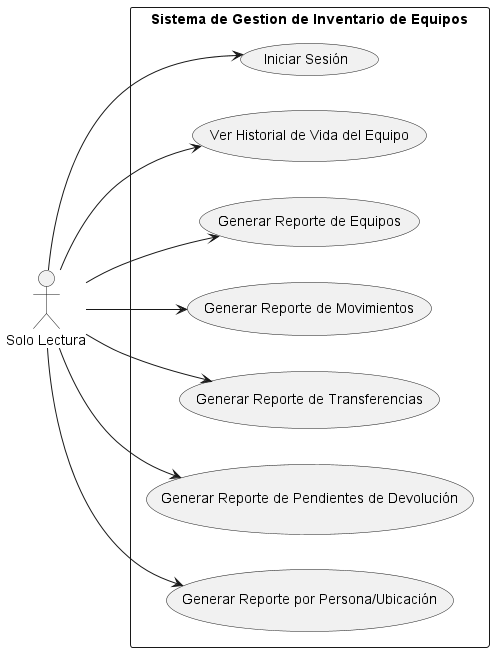
\includegraphics[scale=0.62]{./diagrams/CaseUses/ReadOnly/Solo Lectura.pdf}
\end{figure}
\begin{figure}[H]
    \centering
    \caption{Casos de Uso: Administrador}\label{admin}
    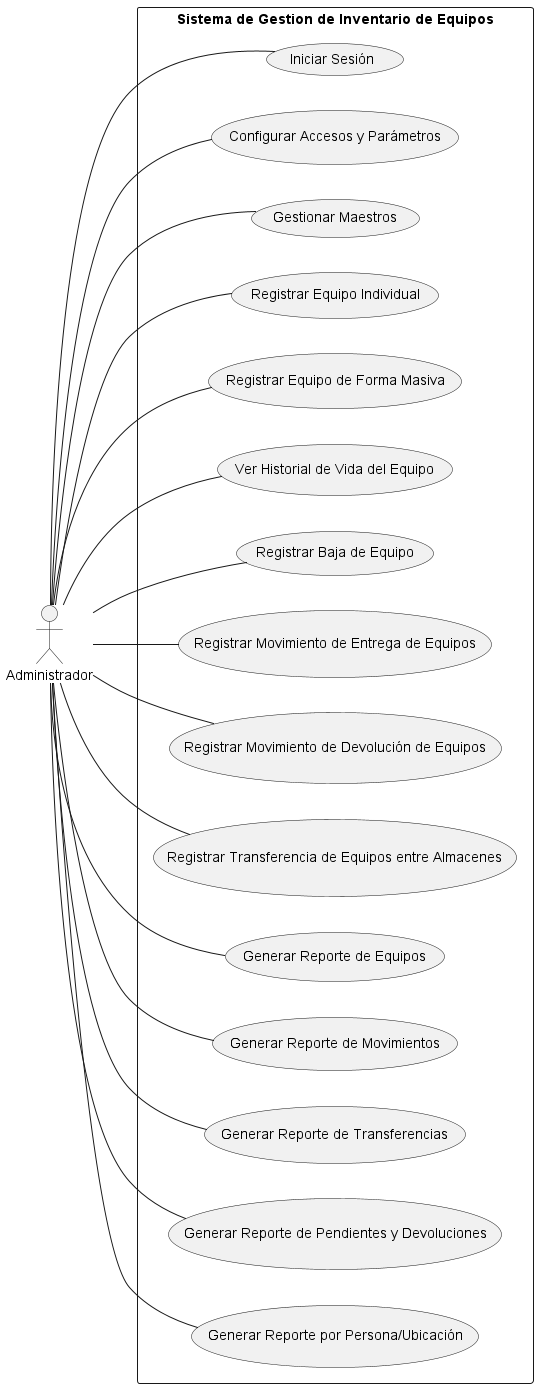
\includegraphics[scale=0.43]{./diagrams/CaseUses/Admin/Administrador.pdf}
\end{figure}
\subsubsection{Especificación de Casos de Uso}
Ahora se detallarán las especificaciones de cada uno de los casos de uso identificados anteriormente. Estas especificaciones proporcionan una
descripción precisa y estructurada de las interacciones entre los actores y el sistema, destacando los flujos de eventos principales, las
precondiciones, postcondiciones, y las excepciones relevantes. La especificación de casos de uso es esencial para guiar el diseño y desarrollo
del módulo, asegurando que todas las funcionalidades requeridas estén claramente definidas y alineadas con los objetivos del sistema.
\newline
\begin{longtable}{@{} p{16.5cm} @{}}
    \caption{Especificación de Caso de Uso: Iniciar Sesión}\label{tab:UC01}                                                             \\ \toprule
    \multicolumn{1}{c}{Caso de uso: Iniciar Sesión}                                                                                     \\ \midrule
    ID:~UC01                                                                                                                            \\ \midrule
    Breve descripción:                                                                                                                  \\
    El usuario se autentica en el sistema utilizando sus credenciales de NextSoft-ERP.                                                  \\ \midrule
    Actores principales:                                                                                                                \\
    Usuario (Administrador, Solo Lector)                                                                                                \\ \midrule
    Actores secundarios:                                                                                                                \\
    Ninguno                                                                                                                             \\ \midrule
    Precondiciones:                                                                                                                     \\
    1. El usuario debe tener una cuenta activa en el NextAdmin.                                                                         \\ \midrule
    Flujo principal:                                                                                                                    \\
    1. El usuario navega a la pantalla de inicio de sesión del módulo de gestión de inventario de equipos.                              \\
    2. El sistema muestra un formulario de inicio de sesión donde el usuario ingresa sus credenciales (nombre de usuario y contraseña). \\
    3. El usuario ingresa sus credenciales y presiona el botón ``Iniciar Sesión''.                                                      \\
    4. El sistema valida las credenciales proporcionadas.                                                                               \\
    5. Si las credenciales son correctas, el sistema autentica al usuario y muestra una pantalla para que elija el almacén.             \\
    6. Una vez elegido el almacén determina su rol (Administrador o Solo Lectura).                                                      \\
    7. El usuario es redirigido a la página principal del módulo con los permisos correspondientes a su rol.                            \\ \midrule
    Postcondiciones:                                                                                                                    \\
    1. El usuario accede al módulo con los permisos correspondientes a su rol.                                                          \\ \midrule
    Flujos alternativos:                                                                                                                \\
    A1- Credenciales incorrectas:                                                                                                       \\
    \hspace{1cm}1. El sistema detecta que las credenciales ingresadas no son correctas.                                                 \\
    \hspace{1cm}2. El sistema muestra un mensaje de error indicando que las credenciales son inválidas.                                 \\
    \hspace{1cm}3. El flujo retorna al paso 2 del flujo principal si el usuario decide intentar nuevamente.                             \\ \bottomrule
\end{longtable}
\newpage
\begin{longtable}{@{} p{16.5cm} @{}}
    \caption{Especificación de Caso de Uso: Configurar Accesos y Parámetros}\label{tab:UC02}                                                         \\ \toprule
    \multicolumn{1}{c}{Caso de uso: Configurar Accesos y Parámetros}                                                                                 \\ \midrule
    ID:~UC02                                                                                                                                         \\ \midrule
    Breve descripción:                                                                                                                               \\
    El administrador configura los usuarios con acceso a los almacenes y define los parámetros del sistema.                                          \\ \midrule
    Actores principales:                                                                                                                             \\
    Administrador                                                                                                                                    \\ \midrule
    Actores secundarios:                                                                                                                             \\
    Ninguno                                                                                                                                          \\ \midrule
    Precondiciones:                                                                                                                                  \\
    1. El administrador debe haber iniciado sesión.                                                                                                  \\ \midrule
    Flujo principal:                                                                                                                                 \\
    1. El administrador navega a la sección de configuración del módulo de gestión de inventario de equipos.                                         \\
    2. El sistema muestra una interfaz con opciones para configurar accesos a almacenes y definir parámetros del sistema.                            \\
    3. El administrador selecciona la opción para gestionar usuarios y asignar permisos de acceso a los almacenes.                                   \\
    4. El administrador elige los usuarios, define su rol (Administrador o Solo Lectura) y asigna los almacenes correspondientes.                    \\
    5. El administrador guarda los cambios realizados.                                                                                               \\
    6. El sistema guarda la configuración de accesos en la base de datos y muestra un mensaje de confirmación.                                       \\
    7. A continuación, el administrador selecciona la opción para definir parámetros generales del módulo (p. ej., familia de productos.).           \\
    8. El administrador ajusta los parámetros necesarios y guarda los cambios.                                                                       \\
    9. El sistema guarda los parámetros en la base de datos y confirma la actualización con un mensaje de éxito.                                     \\ \midrule
    Postcondiciones:                                                                                                                                 \\
    1. Los usuarios y parámetros son configurados correctamente y guardados en el sistema.                                                           \\ \midrule
    Flujos alternativos:                                                                                                                             \\
    A1- Error al guardar configuraciones:                                                                                                            \\
    \hspace{1cm}1. Si ocurre un error durante el guardado de los accesos o parámetros, el sistema muestra un mensaje de error indicando el problema. \\
    \hspace{1cm}2. El administrador tiene la opción de intentar guardar nuevamente o revisar los cambios realizados.                                 \\
    \hspace{1cm}3. El flujo retorna al paso 5 o 8 del flujo principal, dependiendo de la acción que decida tomar el administrador.                   \\ \bottomrule
\end{longtable}
\newpage
\begin{longtable}{@{} p{16.5cm} @{}}
    \caption{Especificación de Caso de Uso: Gestionar Maestros}\label{tab:UC03}                                                                                                              \\ \toprule
    \multicolumn{1}{c}{Caso de uso: Gestionar Maestros}                                                                                                                                      \\ \midrule
    ID:~UC03                                                                                                                                                                                 \\ \midrule
    Breve descripción:                                                                                                                                                                       \\
    El usuario administra los datos maestros, como categorías, marcas, modelos, almacenes, proyectos, ubicaciones y atributos de equipos.                                                    \\ \midrule
    Actores principales:                                                                                                                                                                     \\
    Administrador                                                                                                                                                                            \\ \midrule
    Actores secundarios:                                                                                                                                                                     \\
    Ninguno                                                                                                                                                                                  \\ \midrule
    Precondiciones:                                                                                                                                                                          \\
    1. El administrador debe haber iniciado sesión.                                                                                                                                          \\ \midrule
    Flujo principal:                                                                                                                                                                         \\
    1. El administrador accede a la sección de ``Maestros'' en el módulo de gestión de inventario de equipos.                                                                                \\
    2. El sistema muestra una lista de opciones para administrar diferentes tipos de datos maestros (categorías, marcas, modelos, almacenes, proyectos, ubicaciones y atributos de equipos). \\
    3. El administrador selecciona una de las opciones para gestionar los datos maestros.                                                                                                    \\
    4. El sistema muestra una lista con los registros existentes para el tipo de dato maestro seleccionado.                                                                                  \\
    5. El administrador puede realizar las siguientes acciones:                                                                                                                              \\
    \hspace{1cm}- Registrar un nuevo dato maestro: El administrador introduce la información requerida en un formulario y guarda el nuevo registro.                                          \\
    \hspace{1cm}- Actualizar un dato maestro existente: El administrador selecciona un registro, edita la información y guarda los cambios.                                                  \\
    \hspace{1cm}- Eliminar un dato maestro: El administrador selecciona un registro y lo elimina del sistema.                                                                                \\
    6. El sistema guarda los cambios realizados (registro, actualización o eliminación) en la base de datos y muestra un mensaje de confirmación.                                            \\
    7. El administrador puede repetir el proceso para otros datos maestros o salir de la sección.                                                                                            \\ \midrule
    Postcondiciones:                                                                                                                                                                         \\
    1. Los datos maestros son registrados, actualizados o eliminados en el sistema.                                                                                                          \\ \midrule
    Flujos alternativos:                                                                                                                                                                     \\
    A1- Error al guardar cambios:                                                                                                                                                            \\
    \hspace{1cm}1. Si ocurre un error al intentar registrar, actualizar o eliminar un dato maestro, el sistema muestra un mensaje de error indicando el problema.                            \\
    \hspace{1cm}2. El administrador tiene la opción de intentar la acción nuevamente o revisar los cambios realizados.                                                                       \\
    \hspace{1cm}3. El flujo retorna al paso 5 del flujo principal, dependiendo de la acción que decida tomar el administrador.                                                               \\ \bottomrule
\end{longtable}
\newpage
\begin{longtable}{@{} p{16.5cm} @{}}
    \caption{Especificación de Caso de Uso: Registrar Equipo Individual}\label{tab:UC04}                                                                                                                                                                                       \\ \toprule
    \multicolumn{1}{c}{Caso de uso: Registrar Equipo Individual}                                                                                                                                                                                                               \\ \midrule
    ID:~UC04                                                                                                                                                                                                                                                                   \\ \midrule
    Breve descripción:                                                                                                                                                                                                                                                         \\
    El administrador registra un equipo en el sistema de forma individual.                                                                                                                                                                                                     \\ \midrule
    Actores principales:                                                                                                                                                                                                                                                       \\
    Administrador                                                                                                                                                                                                                                                              \\ \midrule
    Actores secundarios:                                                                                                                                                                                                                                                       \\
    Ninguno                                                                                                                                                                                                                                                                    \\ \midrule
    Precondiciones:                                                                                                                                                                                                                                                            \\
    1. El usuario debe haber iniciado sesión y tener el rol de administrador en el almacén seleccionado.                                                                                                                                                                       \\ \midrule
    Flujo principal:                                                                                                                                                                                                                                                           \\
    1. El administrador accede a la sección de ``Agregar un nuevo equipo'' en el módulo de gestión de inventario de equipos.                                                                                                                                                   \\
    2. El sistema muestra un formulario para el registro individual de un equipo, solicitando información como los datos de la factura, categoría, producto, marca, modelo, número de serie, activo fijo, descripción, fecha y detalle de garantía, atributos y calibraciones. \\
    3. El administrador completa el formulario con la información del equipo.                                                                                                                                                                                                  \\
    4. El administrador revisa la información ingresada y presiona el botón ``Guardar''.                                                                                                                                                                                       \\
    5. El sistema valida la información proporcionada y guarda el nuevo equipo en la base de datos.                                                                                                                                                                            \\
    6. Automáticamente, el sistema genera un movimiento de ingreso vinculado al almacén correspondiente donde se registró el equipo.                                                                                                                                           \\
    7. El sistema muestra un mensaje de confirmación indicando que el equipo ha sido registrado exitosamente.                                                                                                                                                                  \\ \midrule
    Postcondiciones:                                                                                                                                                                                                                                                           \\
    1. El equipo es registrado, y se genera un movimiento de ingreso asociado al almacén.                                                                                                                                                                                      \\ \midrule
    Flujos alternativos:                                                                                                                                                                                                                                                       \\
    A1- Información inválida o incompleta:                                                                                                                                                                                                                                     \\
    \hspace{1cm}1. Si la información ingresada por el administrador es inválida o está incompleta, el sistema muestra un mensaje de error indicando los campos que necesitan corrección.                                                                                       \\
    \hspace{1cm}2. El administrador corrige la información y vuelve a intentar el registro del equipo.                                                                                                                                                                         \\
    \hspace{1cm}3. El flujo retorna al paso 4 del flujo principal.                                                                                                                                                                                                             \\ \bottomrule
\end{longtable}
\newpage
\begin{longtable}{@{} p{16.5cm} @{}}
    \caption{Especificación de Caso de Uso: Registrar Equipo de Forma Masiva}\label{tab:UC05}                                                                          \\ \toprule
    \multicolumn{1}{c}{Caso de uso: Registrar Equipo de Forma Masiva}                                                                                                  \\ \midrule
    ID:~UC05                                                                                                                                                           \\ \midrule
    Breve descripción:                                                                                                                                                 \\
    El administrador carga un archivo EXCEL para registrar múltiples equipos simultáneamente.                                                                          \\ \midrule
    Actores principales:                                                                                                                                               \\
    Administrador                                                                                                                                                      \\ \midrule
    Actores secundarios:                                                                                                                                               \\
    Ninguno                                                                                                                                                            \\ \midrule
    Precondiciones:                                                                                                                                                    \\
    1. El usuario debe haber iniciado sesión y tener el rol de administrador en el almacén seleccionado.                                                               \\
    2. El usuario debe descargar la plantilla EXCEL.                                                                                                                   \\
    3. El usuario debe llenar la plantilla EXCEL con los datos solicitados.                                                                                            \\ \midrule
    Flujo principal:                                                                                                                                                   \\
    1. El administrador accede a la sección de ``Agregar varios desde un EXCEL'' en el módulo de gestión de inventario de equipos.                                     \\
    2. El sistema muestra una opción para cargar un archivo EXCEL con la información de los equipos a registrar.                                                       \\
    3. El administrador selecciona el archivo EXCEL desde su dispositivo y lo carga en el sistema.                                                                     \\
    4. El sistema procesa el archivo, validando que la información esté completa y sea correcta (e.g., formato correcto de número de serie, categorías válidas, etc.). \\
    5. Si el archivo es válido, el sistema muestra la lista de equipos procesados desde el EXCEL.                                                                      \\
    6. El administrador revisa la información y presiona el botón ``Guardar''.                                                                                         \\
    7. Automáticamente, el sistema genera movimientos de ingreso para cada equipo registrado, vinculados al almacén correspondiente.                                   \\
    8. El sistema muestra un mensaje de confirmación indicando que los equipos han sido registrados exitosamente.                                                      \\ \midrule
    Postcondiciones:                                                                                                                                                   \\
    1. Los equipos son registrados masivamente, y se generan los movimientos de ingreso correspondientes.                                                              \\ \midrule
    Flujos alternativos:                                                                                                                                               \\
    A1- Archivo EXCEL inválido o información incorrecta:                                                                                                               \\
    \hspace{1cm}1. Si el archivo EXCEL tiene un formato incorrecto o contiene información inválida, el sistema muestra un mensaje de error.                            \\
    \hspace{1cm}2. El administrador corrige el archivo y lo carga nuevamente en el sistema.                                                                            \\
    \hspace{1cm}3. El flujo retorna al paso 3 del flujo principal.                                                                                                     \\ \bottomrule
\end{longtable}
\newpage
\begin{longtable}{@{} p{16.5cm} @{}}
    \caption{Especificación de Caso de Uso: Ver Historial de Vida del Equipo}\label{tab:UC06}                                                                                           \\ \toprule
    \multicolumn{1}{c}{Caso de uso: Ver Historial de Vida del Equipo}                                                                                                                   \\ \midrule
    ID:~UC06                                                                                                                                                                            \\ \midrule
    Breve descripción:                                                                                                                                                                  \\
    El usuario visualiza el historial de vida de un equipo.                                                                                                                             \\ \midrule
    Actores principales:                                                                                                                                                                \\
    Administrador, Solo Lector                                                                                                                                                          \\ \midrule
    Actores secundarios:                                                                                                                                                                \\
    Ninguno                                                                                                                                                                             \\ \midrule
    Precondiciones:                                                                                                                                                                     \\
    1. El usuario debe haber iniciado sesión.                                                                                                                                           \\ \midrule
    Flujo principal:                                                                                                                                                                    \\
    1. El usuario accede a la sección de ``Ver historial'' en el módulo de gestión de inventario de equipos.                                                                            \\
    2. El sistema recupera la información del equipo seleccionado de la base de datos, incluyendo todos los cambios de estado (e.g., disponible, baja, mantenimiento, asignado).        \\
    3. El sistema muestra el historial completo del equipo en un modal, organizado de manera cronológica.                                                                               \\
    4. El usuario puede revisar el historial detallado, ver cada evento o cambio de estado con su fecha correspondiente, y obtener un panorama completo de la vida útil del equipo.     \\ \midrule
    Postcondiciones:                                                                                                                                                                    \\
    1. El historial del equipo es mostrado en la pantalla.                                                                                                                              \\ \midrule
    Flujos alternativos:                                                                                                                                                                \\
    A1- Equipo no encontrado:                                                                                                                                                           \\
    \hspace{1cm}1. Si el equipo no se encuentra en la base de datos, el sistema muestra un mensaje de error, indicando que no se han encontrado resultados para el equipo seleccionado. \\
    \hspace{1cm}2. El flujo retorna al paso 1 del flujo principal si se realiza una nueva búsqueda.                                                                                     \\
    A2- Error al recuperar datos del historial:                                                                                                                                         \\
    \hspace{1cm}1. Si ocurre un error al intentar recuperar los datos del historial del equipo, el sistema muestra un mensaje de error indicando el problema.                           \\
    \hspace{1cm}2. Si el problema persiste, el usuario puede contactar al soporte técnico para asistencia. El flujo puede continuar con una nueva búsqueda o finalizar el caso de uso.  \\ \bottomrule
\end{longtable}
\newpage
\begin{longtable}{@{} p{16.5cm} @{}}
    \caption{Especificación de Caso de Uso: Registrar Baja de Equipo}\label{tab:UC07}                                                                                                                                                 \\ \toprule
    \multicolumn{1}{c}{Caso de uso: Registrar Baja de Equipo}                                                                                                                                                                         \\ \midrule
    ID:~UC07                                                                                                                                                                                                                          \\ \midrule
    Breve descripción:                                                                                                                                                                                                                \\
    El administrador registra la baja de un equipo, especificando el motivo.                                                                                                                                                          \\ \midrule
    Actores principales:                                                                                                                                                                                                              \\
    Administrador                                                                                                                                                                                                                     \\ \midrule
    Actores secundarios:                                                                                                                                                                                                              \\
    Ninguno                                                                                                                                                                                                                           \\ \midrule
    Precondiciones:                                                                                                                                                                                                                   \\
    1. El usuario debe haber iniciado sesión y tener el rol de administrador en el almacén seleccionado.                                                                                                                              \\
    2. El equipo debe estar en estado ``Disponible''.                                                                                                                                                                                 \\ \midrule
    Flujo principal:                                                                                                                                                                                                                  \\
    1. El administrador accede a la sección de ``Equipos'' en el módulo de gestión de inventario de equipos.                                                                                                                          \\
    2. El administrador selecciona el equipo que será dado de baja.                                                                                                                                                                   \\
    3. El administrador especifica el motivo de la baja para el equipo seleccionado.                                                                                                                                                  \\
    4. El administrador confirma la baja del equipo.                                                                                                                                                                                  \\
    5. El sistema verifica que el equipo seleccionado está actualmente en el almacén y en un estado que permite la baja (e.g., ``Disponible'').                                                                                       \\
    6. El sistema actualiza el estado del equipo en la base de datos, cambiándolo a ``Baja'', junto con el motivo especificado.                                                                                                       \\                                                                                                                     \\
    8. El sistema muestra una confirmación de que la baja del equipo se ha registrado correctamente.                                                                                                                                  \\ \midrule
    Postcondiciones:                                                                                                                                                                                                                  \\
    1. El equipo es dado de baja, y se actualiza su estado a ``Baja'' en el sistema.                                                                                                                                                  \\ \midrule
    Flujos alternativos:                                                                                                                                                                                                              \\
    A1- Equipo no disponible para baja:                                                                                                                                                                                               \\
    \hspace{1cm}1. Si el equipo seleccionado no está disponible para la baja (e.g., en estado ``Asignado'', ``Mantenimiento'' o ya dado de baja), el sistema muestra un mensaje de error indicando que no se puede completar la baja. \\
    \hspace{1cm}3. El flujo retorna al paso 2 del flujo principal.                                                                                                                                                                    \\
    A2- Error en la base de datos:                                                                                                                                                                                                    \\
    \hspace{1cm}1. Si ocurre un error al intentar actualizar el estado del equipo o registrar la baja en la base de datos, el sistema muestra un mensaje de error indicando el problema.                                              \\
    \hspace{1cm}2. El administrador puede intentar registrar nuevamente la baja, o contactar al soporte técnico si el problema persiste.                                                                                              \\
    \hspace{1cm}3. El flujo puede continuar con una nueva tentativa de registro o finalizar el caso de uso.                                                                                                                           \\ \bottomrule
\end{longtable}
\newpage
\begin{longtable}{@{} p{16.5cm} @{}}
    \caption{Especificación de Caso de Uso: Registrar Movimiento de Entrega de Equipos}\label{tab:UC08}                                                                                                                    \\ \toprule
    \multicolumn{1}{c}{Caso de uso: Registrar Movimiento de Entrega de Equipos}                                                                                                                                            \\ \midrule
    ID:~UC08                                                                                                                                                                                                               \\ \midrule
    Breve descripción:                                                                                                                                                                                                     \\
    El administrador registra la entrega de uno o varios equipos a un responsable.                                                                                                                                         \\ \midrule
    Actores principales:                                                                                                                                                                                                   \\
    Administrador                                                                                                                                                                                                          \\ \midrule
    Actores secundarios:                                                                                                                                                                                                   \\
    Ninguno                                                                                                                                                                                                                \\ \midrule
    Precondiciones:                                                                                                                                                                                                        \\
    1. El usuario debe haber iniciado sesión y tener el rol de administrador en el almacén seleccionado.                                                                                                                   \\ \midrule
    Flujo principal:                                                                                                                                                                                                       \\
    1. El administrador accede a la sección de ``Registrar entrega'' en el módulo de gestión de inventario de equipos.                                                                                                     \\
    2. El administrador selecciona uno o varios equipos que serán entregados.                                                                                                                                              \\
    3. El administrador asigna un responsable o una ubicación para los equipos seleccionados, además de un proyecto, sector y un motivo.                                                                                   \\
    4. El sistema verifica que los equipos seleccionados estén disponibles (estado ``Disponible'').                                                                                                                        \\
    5. El administrador confirma la entrega de los equipos.                                                                                                                                                                \\
    6. El sistema actualiza el estado de los equipos a ``Asignado'' y registra el movimiento de entrega en la base de datos, asociándolo al responsable asignado.                                                          \\
    7. El sistema muestra una confirmación de que la entrega se ha registrado correctamente.                                                                                                                               \\
    8. El administrador puede visualizar un resumen de la entrega o registrar una nueva entrega.                                                                                                                           \\ \midrule
    Postcondiciones:                                                                                                                                                                                                       \\
    1. El resumen de la entrega es mostrado en la pantalla.                                                                                                                                                                \\ \midrule
    Flujos alternativos:                                                                                                                                                                                                   \\
    A1- Equipo no disponible:                                                                                                                                                                                              \\
    \hspace{1cm}1. Si alguno de los equipos seleccionados no está disponible (e.g., ya asignado, en mantenimiento, o dado de baja), el sistema muestra un mensaje de error indicando que no se puede completar la entrega. \\
    \hspace{1cm}2. El administrador puede optar por deseleccionar los equipos no disponibles y continuar con la entrega de los equipos restantes.                                                                          \\
    \hspace{1cm}3. El flujo retorna al paso 5 del flujo principal si el administrador decide continuar.                                                                                                                    \\
    A2- Error en la base de datos:                                                                                                                                                                                         \\
    \hspace{1cm}1. Si ocurre un error al intentar actualizar el estado de los equipos o registrar el movimiento de entrega en la base de datos, el sistema muestra un mensaje de error indicando el problema.              \\
    \hspace{1cm}2. El administrador puede intentar registrar nuevamente la entrega, o contactar al soporte técnico si el problema persiste.                                                                                \\
    \hspace{1cm}3. El flujo puede continuar con una nueva tentativa de registro o finalizar el caso de uso.                                                                                                                \\ \bottomrule
\end{longtable}
\newpage
\begin{longtable}{@{} p{16.5cm} @{}}
    \caption{Especificación de Caso de Uso: Registrar Movimiento de Devolución de Equipos}\label{tab:UC09}                                                                                                                           \\ \toprule
    \multicolumn{1}{c}{Caso de uso: Registrar Movimiento de Devolución de Equipos}                                                                                                                                                   \\ \midrule
    ID:~UC09                                                                                                                                                                                                                         \\ \midrule
    Breve descripción:                                                                                                                                                                                                               \\
    El administrador registra la devolución de uno o varios equipos al almacén.                                                                                                                                                      \\ \midrule
    Actores principales:                                                                                                                                                                                                             \\
    Administrador                                                                                                                                                                                                                    \\ \midrule
    Actores secundarios:                                                                                                                                                                                                             \\
    Ninguno                                                                                                                                                                                                                          \\ \midrule
    Precondiciones:                                                                                                                                                                                                                  \\
    1. El usuario debe haber iniciado sesión y tener el rol de administrador en el almacén seleccionado.                                                                                                                             \\
    2. El usuario debe haber seleccionado los equipos a devolver.                                                                                                                                                                    \\
    3. Los equipos seleccionados deben tener a un solo responsable.                                                                                                                                                                  \\ \midrule
    Flujo principal:                                                                                                                                                                                                                 \\
    1. El administrador accede a la sección de ``Registrar devolución'' en el módulo de gestión de inventario de equipos.                                                                                                            \\
    2. El administrador escribe el motivo de la devolución de los equipos.                                                                                                                                                           \\
    3. El administrador confirma el estado físico del equipo y escribe una observación por cada equipo si fuera necesario.                                                                                                           \\
    4. El sistema verifica que los equipos seleccionados están actualmente asignados (estado ``Asignado'').                                                                                                                          \\
    5. El administrador confirma la devolución de los equipos.                                                                                                                                                                       \\
    6. El sistema actualiza el estado de los equipos a ``Disponible'' y registra el movimiento de devolución en la base de datos, liberando la asignación al responsable anterior.                                                   \\
    7. El sistema muestra una confirmación de que la devolución se ha registrado correctamente.                                                                                                                                      \\
    8. El administrador puede visualizar un resumen de la devolución o registrar una nueva devolución.                                                                                                                               \\ \midrule
    Postcondiciones:                                                                                                                                                                                                                 \\
    1. Los equipos son devueltos, y se actualiza el estado a ``Activo''.                                                                                                                                                             \\ \midrule
    Flujos alternativos:                                                                                                                                                                                                             \\
    A1- Equipo no asignado:                                                                                                                                                                                                          \\
    \hspace{1cm}1. Si alguno de los equipos seleccionados no está asignado (e.g., ya en estado ``Activo'', ``Baja'', o ``Mantenimiento''), el sistema muestra un mensaje de error indicando que no se puede completar la devolución. \\
    \hspace{1cm}3. El flujo retorna al paso 1 del flujo principal.                                                                                                                                                                   \\
    A2- Error en la base de datos:                                                                                                                                                                                                   \\
    \hspace{1cm}1. Si ocurre un error al intentar actualizar el estado de los equipos o registrar el movimiento de devolución en la base de datos, el sistema muestra un mensaje de error indicando el problema.                     \\
    \hspace{1cm}2. El administrador puede intentar registrar nuevamente la devolución, o contactar al soporte técnico si el problema persiste.                                                                                       \\
    \hspace{1cm}3. El flujo puede continuar con una nueva tentativa de registro o finalizar el caso de uso.                                                                                                                          \\ \bottomrule
\end{longtable}
\newpage
\begin{longtable}{@{} p{16.5cm} @{}}
    \caption{Especificación de Caso de Uso: Registrar Transferencia de Equipos entre Almacenes}\label{tab:UC010}                                                                                                                           \\ \toprule
    \multicolumn{1}{c}{Caso de uso: Registrar Transferencia de Equipos entre Almacenes}                                                                                                                                                    \\ \midrule
    ID:~UC010                                                                                                                                                                                                                              \\ \midrule
    Breve descripción:                                                                                                                                                                                                                     \\
    El administrador transfiere uno o varios equipos de un almacén a otro.                                                                                                                                                                 \\ \midrule
    Actores principales:                                                                                                                                                                                                                   \\
    Administrador                                                                                                                                                                                                                          \\ \midrule
    Actores secundarios:                                                                                                                                                                                                                   \\
    Ninguno                                                                                                                                                                                                                                \\ \midrule
    Precondiciones:                                                                                                                                                                                                                        \\
    1. El usuario debe haber iniciado sesión y tener el rol de administrador en el almacén seleccionado (origen).                                                                                                                          \\ \midrule
    Flujo principal:                                                                                                                                                                                                                       \\
    1. El administrador accede a la sección de ``Registrar transferencia'' en el módulo de gestión de inventario de equipos.                                                                                                               \\
    2. El administrador selecciona el almacén de destino para la transferencia.                                                                                                                                                            \\
    3. El administrador selecciona uno o varios equipos que serán transferidos del almacén de origen al almacén de destino.                                                                                                                \\
    4. El administrador confirma la transferencia de los equipos.                                                                                                                                                                          \\
    5. El sistema verifica que los equipos seleccionados están actualmente en el almacén de origen y en un estado que permite la transferencia (e.g., ``Disponible'').                                                                     \\
    6. El sistema actualiza el estado de los equipos en la base de datos, registrando la salida del almacén de origen y la entrada en el almacén de destino.                                                                               \\
    7. El sistema genera los movimientos correspondientes en la base de datos, registrando la transferencia para cada equipo.                                                                                                              \\
    8. El sistema muestra una confirmación de que la transferencia se ha registrado correctamente.                                                                                                                                         \\
    9. El administrador puede visualizar un resumen de la transferencia o registrar una nueva transferencia.                                                                                                                               \\ \midrule
    Postcondiciones:                                                                                                                                                                                                                       \\
    1. Los equipos son transferidos, y se generan los movimientos correspondientes en el sistema.                                                                                                                                          \\ \midrule
    Flujos alternativos:                                                                                                                                                                                                                   \\
    A1- Equipo no disponible para trasferencia:                                                                                                                                                                                            \\
    \hspace{1cm}1. Si alguno de los equipos seleccionados no está disponible para la transferencia (e.g., en estado ``Baja'' o ``Asignado''), el sistema muestra un mensaje de error indicando que no se puede completar la transferencia. \\
    \hspace{1cm}2. El administrador puede optar por deseleccionar los equipos no transferibles y continuar con la transferencia de los equipos restantes.                                                                                  \\
    \hspace{1cm}3. El flujo retorna al paso 5 del flujo principal si el administrador decide continuar.                                                                                                                                    \\
    A2- Error en la base de datos:                                                                                                                                                                                                         \\
    \hspace{1cm}1. Si ocurre un error al intentar registrar los movimientos de transferencia en la base de datos, el sistema muestra un mensaje de error indicando el problema.                                                            \\
    \hspace{1cm}2. El administrador puede intentar registrar nuevamente la transferencia, o contactar al soporte técnico si el problema persiste.                                                                                          \\
    \hspace{1cm}3. El flujo puede continuar con una nueva tentativa de registro o finalizar el caso de uso.                                                                                                                                \\ \bottomrule
\end{longtable}
\newpage
\begin{longtable}{@{} p{16.5cm} @{}}
    \caption{Especificación de Caso de Uso: Generar Reporte de Equipos}\label{tab:UC011}                                                                                                                                                                                       \\ \toprule
    \multicolumn{1}{c}{Caso de uso: Generar Reporte de Equipos}                                                                                                                                                                                                                \\ \midrule
    ID:~UC011                                                                                                                                                                                                                                                                  \\ \midrule
    Breve descripción:                                                                                                                                                                                                                                                         \\
    El usuario genera un reporte que muestra todos los equipos registrados en el sistema, filtrando por categoría, marca, equipo, estado, entre otros criterios.                                                                                                               \\ \midrule
    Actores principales:                                                                                                                                                                                                                                                       \\
    Administrador, Solo Lector                                                                                                                                                                                                                                                 \\ \midrule
    Actores secundarios:                                                                                                                                                                                                                                                       \\
    Ninguno                                                                                                                                                                                                                                                                    \\ \midrule
    Precondiciones:                                                                                                                                                                                                                                                            \\
    1. El usuario debe haber iniciado sesión.                                                                                                                                                                                                                                  \\ \midrule
    Flujo principal:                                                                                                                                                                                                                                                           \\
    1. El usuario accede a la sección de ``Reporte de equipos'' en el módulo de gestión de inventario de equipos.                                                                                                                                                              \\
    2. El sistema presenta una interfaz en la que el usuario puede seleccionar los filtros deseados, como estado del equipo, categoría, fechas, entre otros.                                                                                                                   \\
    3. El usuario selecciona los criterios de filtrado y el formato de exportación del reporte (e.g., Excel, Listado).                                                                                                                                                         \\
    4. El usuario confirma la generación del reporte.                                                                                                                                                                                                                          \\
    5. El sistema consulta la base de datos para recuperar la información de los equipos que cumplen con los criterios de filtrado especificados.                                                                                                                              \\
    6. El sistema genera el reporte con la información obtenida, presentándolo en pantalla para su revisión.                                                                                                                                                                   \\
    7. Si el usuario seleccionó un formato de exportación, el sistema genera un archivo en el formato especificado.                                                                                                                                                            \\
    8. El usuario revisa el reporte y puede optar por guardarlo, imprimirlo o realizar una nueva consulta.                                                                                                                                                                     \\ \midrule
    Postcondiciones:                                                                                                                                                                                                                                                           \\
    1. El reporte es generado y presentado en pantalla o exportado en un formato seleccionable (e.g., Excel).                                                                                                                                                                  \\ \midrule
    Flujos alternativos:                                                                                                                                                                                                                                                       \\
    A1- Filtros inválidos o sin resultados:                                                                                                                                                                                                                                    \\
    \hspace{1cm}1. Si el usuario selecciona un conjunto de filtros que no devuelve ningún resultado (e.g., no hay equipos que coincidan con los criterios seleccionados), el sistema muestra un mensaje informando que no se encontraron datos para los filtros seleccionados. \\
    \hspace{1cm}2. El usuario puede optar por modificar los filtros y realizar una nueva consulta.                                                                                                                                                                             \\
    \hspace{1cm}3. El flujo retorna al paso 3 del flujo principal si el usuario decide ajustar los filtros.                                                                                                                                                                    \\
    A2- Error en la generación del reporte:                                                                                                                                                                                                                                    \\
    \hspace{1cm}1. Si ocurre un error durante la generación del reporte (e.g., problemas con la conexión a la base de datos o error en la exportación del archivo), el sistema muestra un mensaje de error indicando la naturaleza del problema.                               \\
    \hspace{1cm}2. El usuario puede intentar generar el reporte nuevamente, seleccionar un conjunto de filtros diferente, o contactar al soporte técnico si el problema persiste.                                                                                              \\
    \hspace{1cm}3. El flujo puede continuar con una nueva tentativa de generación o finalizar el caso de uso.                                                                                                                                                                  \\ \bottomrule
\end{longtable}
\newpage
\begin{longtable}{@{} p{16.5cm} @{}}
    \caption{Especificación de Caso de Uso: Generar Reporte de Movimientos}\label{tab:UC012}                                                                                                                                                                                       \\ \toprule
    \multicolumn{1}{c}{Caso de uso: Generar Reporte de Movimientos}                                                                                                                                                                                                                \\ \midrule
    ID:~UC012                                                                                                                                                                                                                                                                      \\ \midrule
    Breve descripción:                                                                                                                                                                                                                                                             \\
    El usuario genera un reporte detallado de los movimientos de equipos, incluyendo entregas, devoluciones y transferencias.                                                                                                                                                      \\ \midrule
    Actores principales:                                                                                                                                                                                                                                                           \\
    Administrador, Solo Lector                                                                                                                                                                                                                                                     \\ \midrule
    Actores secundarios:                                                                                                                                                                                                                                                           \\
    Ninguno                                                                                                                                                                                                                                                                        \\ \midrule
    Precondiciones:                                                                                                                                                                                                                                                                \\
    1. El usuario debe haber iniciado sesión.                                                                                                                                                                                                                                      \\ \midrule
    Flujo principal:                                                                                                                                                                                                                                                               \\
    1. El usuario accede a la sección de ``Reporte de movimientos'' en el módulo de gestión de inventario de equipos.                                                                                                                                                              \\
    2. El sistema presenta una interfaz en la que el usuario puede seleccionar los filtros deseados, como tipo de movimiento, responsable, almacén, categoría, fechas, entre otros.                                                                                                \\
    3. El usuario selecciona los criterios de filtrado y el formato de exportación del reporte (e.g., Excel, Listado).                                                                                                                                                             \\
    4. El usuario confirma la generación del reporte.                                                                                                                                                                                                                              \\
    5. El sistema consulta la base de datos para recuperar la información de los movimientos que cumplen con los criterios de filtrado especificados.                                                                                                                              \\
    6. El sistema genera el reporte con la información obtenida, presentándolo en pantalla para su revisión.                                                                                                                                                                       \\
    7. Si el usuario seleccionó un formato de exportación, el sistema genera un archivo en el formato especificado.                                                                                                                                                                \\
    8. El usuario revisa el reporte y puede optar por guardarlo, imprimirlo o realizar una nueva consulta.                                                                                                                                                                         \\ \midrule
    Postcondiciones:                                                                                                                                                                                                                                                               \\
    1. El reporte es generado y presentado en pantalla o exportado en un formato seleccionable (e.g., Excel).                                                                                                                                                                      \\ \midrule
    Flujos alternativos:                                                                                                                                                                                                                                                           \\
    A1- Filtros inválidos o sin resultados:                                                                                                                                                                                                                                        \\
    \hspace{1cm}1. Si el usuario selecciona un conjunto de filtros que no devuelve ningún resultado (e.g., no hay movimientos que coincidan con los criterios seleccionados), el sistema muestra un mensaje informando que no se encontraron datos para los filtros seleccionados. \\
    \hspace{1cm}2. El usuario puede optar por modificar los filtros y realizar una nueva consulta.                                                                                                                                                                                 \\
    \hspace{1cm}3. El flujo retorna al paso 3 del flujo principal si el usuario decide ajustar los filtros.                                                                                                                                                                        \\
    A2- Error en la generación del reporte:                                                                                                                                                                                                                                        \\
    \hspace{1cm}1. Si ocurre un error durante la generación del reporte (e.g., problemas con la conexión a la base de datos o error en la exportación del archivo), el sistema muestra un mensaje de error indicando la naturaleza del problema.                                   \\
    \hspace{1cm}2. El usuario puede intentar generar el reporte nuevamente, seleccionar un conjunto de filtros diferente, o contactar al soporte técnico si el problema persiste.                                                                                                  \\
    \hspace{1cm}3. El flujo puede continuar con una nueva tentativa de generación o finalizar el caso de uso.                                                                                                                                                                      \\ \bottomrule
\end{longtable}
\newpage
\begin{longtable}{@{} p{16.5cm} @{}}
    \caption{Especificación de Caso de Uso: Generar Reporte de Transferencias}\label{tab:UC013}                                                                                                                                                                                       \\ \toprule
    \multicolumn{1}{c}{Caso de uso: Generar Reporte de Transferencias}                                                                                                                                                                                                                \\ \midrule
    ID:~UC013                                                                                                                                                                                                                                                                         \\ \midrule
    Breve descripción:                                                                                                                                                                                                                                                                \\
    El usuario genera un reporte detallado de las transferencias de equipos, filtrando por almacén de origen y almacén de destino.                                                                                                                                                    \\ \midrule
    Actores principales:                                                                                                                                                                                                                                                              \\
    Administrador, Solo Lector                                                                                                                                                                                                                                                        \\ \midrule
    Actores secundarios:                                                                                                                                                                                                                                                              \\
    Ninguno                                                                                                                                                                                                                                                                           \\ \midrule
    Precondiciones:                                                                                                                                                                                                                                                                   \\
    1. El usuario debe haber iniciado sesión.                                                                                                                                                                                                                                         \\ \midrule
    Flujo principal:                                                                                                                                                                                                                                                                  \\
    1. El usuario accede a la sección de ``Reporte de transferencias'' en el módulo de gestión de inventario de equipos.                                                                                                                                                              \\
    2. El sistema presenta una interfaz en la que el usuario puede seleccionar los filtros deseados, como almacén de origen, almacén de destino y fechas.                                                                                                                             \\
    3. El usuario selecciona los criterios de filtrado y el formato de exportación del reporte (e.g., Excel, Listado).                                                                                                                                                                \\
    4. El usuario confirma la generación del reporte.                                                                                                                                                                                                                                 \\
    5. El sistema consulta la base de datos para recuperar la información de las transferencias que cumplen con los criterios de filtrado especificados.                                                                                                                              \\
    6. El sistema genera el reporte con la información obtenida, presentándolo en pantalla para su revisión.                                                                                                                                                                          \\
    7. Si el usuario seleccionó un formato de exportación, el sistema genera un archivo en el formato especificado.                                                                                                                                                                   \\
    8. El usuario revisa el reporte y puede optar por guardarlo, imprimirlo o realizar una nueva consulta.                                                                                                                                                                            \\ \midrule
    Postcondiciones:                                                                                                                                                                                                                                                                  \\
    1. El reporte es generado y presentado en pantalla o exportado en un formato seleccionable (e.g., Excel).                                                                                                                                                                         \\ \midrule
    Flujos alternativos:                                                                                                                                                                                                                                                              \\
    A1- Filtros inválidos o sin resultados:                                                                                                                                                                                                                                           \\
    \hspace{1cm}1. Si el usuario selecciona un conjunto de filtros que no devuelve ningún resultado (e.g., no hay transferencias que coincidan con los criterios seleccionados), el sistema muestra un mensaje informando que no se encontraron datos para los filtros seleccionados. \\
    \hspace{1cm}2. El usuario puede optar por modificar los filtros y realizar una nueva consulta.                                                                                                                                                                                    \\
    \hspace{1cm}3. El flujo retorna al paso 3 del flujo principal si el usuario decide ajustar los filtros.                                                                                                                                                                           \\
    A2- Error en la generación del reporte:                                                                                                                                                                                                                                           \\
    \hspace{1cm}1. Si ocurre un error durante la generación del reporte (e.g., problemas con la conexión a la base de datos o error en la exportación del archivo), el sistema muestra un mensaje de error indicando la naturaleza del problema.                                      \\
    \hspace{1cm}2. El usuario puede intentar generar el reporte nuevamente, seleccionar un conjunto de filtros diferente, o contactar al soporte técnico si el problema persiste.                                                                                                     \\
    \hspace{1cm}3. El flujo puede continuar con una nueva tentativa de generación o finalizar el caso de uso.                                                                                                                                                                         \\ \bottomrule
\end{longtable}
\newpage
\begin{longtable}{@{} p{16.5cm} @{}}
    \caption{Especificación de Caso de Uso: Generar Reporte de Pendientes de Devolución}\label{tab:UC014}                                                                                                                                                                          \\ \toprule
    \multicolumn{1}{c}{Caso de uso: Generar Reporte de Pendientes de Devolución}                                                                                                                                                                                                   \\ \midrule
    ID:~UC014                                                                                                                                                                                                                                                                      \\ \midrule
    Breve descripción:                                                                                                                                                                                                                                                             \\
    El usuario genera un reporte que lista los equipos devueltos y pendientes de devolución.                                                                                                                                                                                       \\ \midrule
    Actores principales:                                                                                                                                                                                                                                                           \\
    Administrador, Solo Lector                                                                                                                                                                                                                                                     \\ \midrule
    Actores secundarios:                                                                                                                                                                                                                                                           \\
    Ninguno                                                                                                                                                                                                                                                                        \\ \midrule
    Precondiciones:                                                                                                                                                                                                                                                                \\
    1. El usuario debe haber iniciado sesión.                                                                                                                                                                                                                                      \\ \midrule
    Flujo principal:                                                                                                                                                                                                                                                               \\
    1. El usuario accede a la sección de ``Reporte de pendientes y devoluciones'' en el módulo de gestión de inventario de equipos.                                                                                                                                                \\
    2. El sistema presenta una interfaz en la que el usuario puede seleccionar los filtros deseados, como almacén, proyecto, sector, ubicación, responsable, tipo (pendiente o devuelto) y fechas.                                                                                 \\
    3. El usuario selecciona los criterios de filtrado y el formato de exportación del reporte (e.g., Excel, Listado).                                                                                                                                                             \\
    4. El usuario confirma la generación del reporte.                                                                                                                                                                                                                              \\
    5. El sistema consulta la base de datos para recuperar la información de los movimientos que cumplen con los criterios de filtrado especificados.                                                                                                                              \\
    6. El sistema genera el reporte con la información obtenida, presentándolo en pantalla para su revisión.                                                                                                                                                                       \\
    7. Si el usuario seleccionó un formato de exportación, el sistema genera un archivo en el formato especificado.                                                                                                                                                                \\
    8. El usuario revisa el reporte y puede optar por guardarlo, imprimirlo o realizar una nueva consulta.                                                                                                                                                                         \\ \midrule
    Postcondiciones:                                                                                                                                                                                                                                                               \\
    1. El reporte es generado y presentado en pantalla o exportado en un formato seleccionable (e.g., Excel).                                                                                                                                                                      \\ \midrule
    Flujos alternativos:                                                                                                                                                                                                                                                           \\
    A1- Filtros inválidos o sin resultados:                                                                                                                                                                                                                                        \\
    \hspace{1cm}1. Si el usuario selecciona un conjunto de filtros que no devuelve ningún resultado (e.g., no hay movimientos que coincidan con los criterios seleccionados), el sistema muestra un mensaje informando que no se encontraron datos para los filtros seleccionados. \\
    \hspace{1cm}2. El usuario puede optar por modificar los filtros y realizar una nueva consulta.                                                                                                                                                                                 \\
    \hspace{1cm}3. El flujo retorna al paso 3 del flujo principal si el usuario decide ajustar los filtros.                                                                                                                                                                        \\
    A2- Error en la generación del reporte:                                                                                                                                                                                                                                        \\
    \hspace{1cm}1. Si ocurre un error durante la generación del reporte (e.g., problemas con la conexión a la base de datos o error en la exportación del archivo), el sistema muestra un mensaje de error indicando la naturaleza del problema.                                   \\
    \hspace{1cm}2. El usuario puede intentar generar el reporte nuevamente, seleccionar un conjunto de filtros diferente, o contactar al soporte técnico si el problema persiste.                                                                                                  \\
    \hspace{1cm}3. El flujo puede continuar con una nueva tentativa de generación o finalizar el caso de uso.                                                                                                                                                                      \\ \bottomrule
\end{longtable}
\newpage
\begin{longtable}{@{} p{16.5cm} @{}}
    \caption{Especificación de Caso de Uso: Generar Reporte por Persona/Ubicación}\label{tab:UC015}                                                                                                                                                                            \\ \toprule
    \multicolumn{1}{c}{Caso de uso: Generar Reporte por Persona/Ubicación}                                                                                                                                                                                                     \\ \midrule
    ID:~UC015                                                                                                                                                                                                                                                                  \\ \midrule
    Breve descripción:                                                                                                                                                                                                                                                         \\
    El usuario genera un reporte que muestra todos los equipos asignados a un trabajador específico o a una ubicación determinada.                                                                                                                                             \\ \midrule
    Actores principales:                                                                                                                                                                                                                                                       \\
    Administrador, Solo Lector                                                                                                                                                                                                                                                 \\ \midrule
    Actores secundarios:                                                                                                                                                                                                                                                       \\
    Ninguno                                                                                                                                                                                                                                                                    \\ \midrule
    Precondiciones:                                                                                                                                                                                                                                                            \\
    1. El usuario debe haber iniciado sesión.                                                                                                                                                                                                                                  \\ \midrule
    Flujo principal:                                                                                                                                                                                                                                                           \\
    1. El usuario accede a la sección de ``Reporte de persona/ubicación'' en el módulo de gestión de inventario de equipos.                                                                                                                                                    \\
    2. El sistema presenta una interfaz en la que el usuario puede seleccionar los filtros deseados, como ubicación, responsable o ambos.                                                                                                                                      \\
    3. El usuario selecciona los criterios de filtrado y el formato de exportación del reporte (e.g., Excel, Listado).                                                                                                                                                         \\
    4. El usuario confirma la generación del reporte.                                                                                                                                                                                                                          \\
    5. El sistema consulta la base de datos para recuperar la información de los equipos que cumplen con los criterios de filtrado especificados.                                                                                                                              \\
    6. El sistema genera el reporte con la información obtenida, presentándolo en pantalla para su revisión.                                                                                                                                                                   \\
    7. Si el usuario seleccionó un formato de exportación, el sistema genera un archivo en el formato especificado.                                                                                                                                                            \\
    8. El usuario revisa el reporte y puede optar por guardarlo, imprimirlo o realizar una nueva consulta.                                                                                                                                                                     \\ \midrule
    Postcondiciones:                                                                                                                                                                                                                                                           \\
    1. El reporte es generado y presentado en pantalla o exportado en un formato seleccionable (e.g., Excel).                                                                                                                                                                  \\ \midrule
    Flujos alternativos:                                                                                                                                                                                                                                                       \\
    A1- Filtros inválidos o sin resultados:                                                                                                                                                                                                                                    \\
    \hspace{1cm}1. Si el usuario selecciona un conjunto de filtros que no devuelve ningún resultado (e.g., no hay equipos que coincidan con los criterios seleccionados), el sistema muestra un mensaje informando que no se encontraron datos para los filtros seleccionados. \\
    \hspace{1cm}2. El usuario puede optar por modificar los filtros y realizar una nueva consulta.                                                                                                                                                                             \\
    \hspace{1cm}3. El flujo retorna al paso 3 del flujo principal si el usuario decide ajustar los filtros.                                                                                                                                                                    \\
    A2- Error en la generación del reporte:                                                                                                                                                                                                                                    \\
    \hspace{1cm}1. Si ocurre un error durante la generación del reporte (e.g., problemas con la conexión a la base de datos o error en la exportación del archivo), el sistema muestra un mensaje de error indicando la naturaleza del problema.                               \\
    \hspace{1cm}2. El usuario puede intentar generar el reporte nuevamente, seleccionar un conjunto de filtros diferente, o contactar al soporte técnico si el problema persiste.                                                                                              \\
    \hspace{1cm}3. El flujo puede continuar con una nueva tentativa de generación o finalizar el caso de uso.                                                                                                                                                                  \\ \bottomrule
\end{longtable}
\newpage
\subsubsection{Diagramas de Clases}
\begin{figure}[H]
    \centering
    \caption{Clases: Entidades}
    \includegraphics[width=21cm, height=16.5cm, angle=90]{./diagrams/Classes/Entities/Entities.pdf}
\end{figure}
\begin{figure}[H]
    \centering
    \caption{Clases: DTO}
    \includegraphics[width=16.5cm, height=21cm, angle=0]{./diagrams/Classes/DTO/DTO.pdf}
\end{figure}
\begin{figure}[H]
    \centering
    \caption{Clases: Lógica de Negocio}
    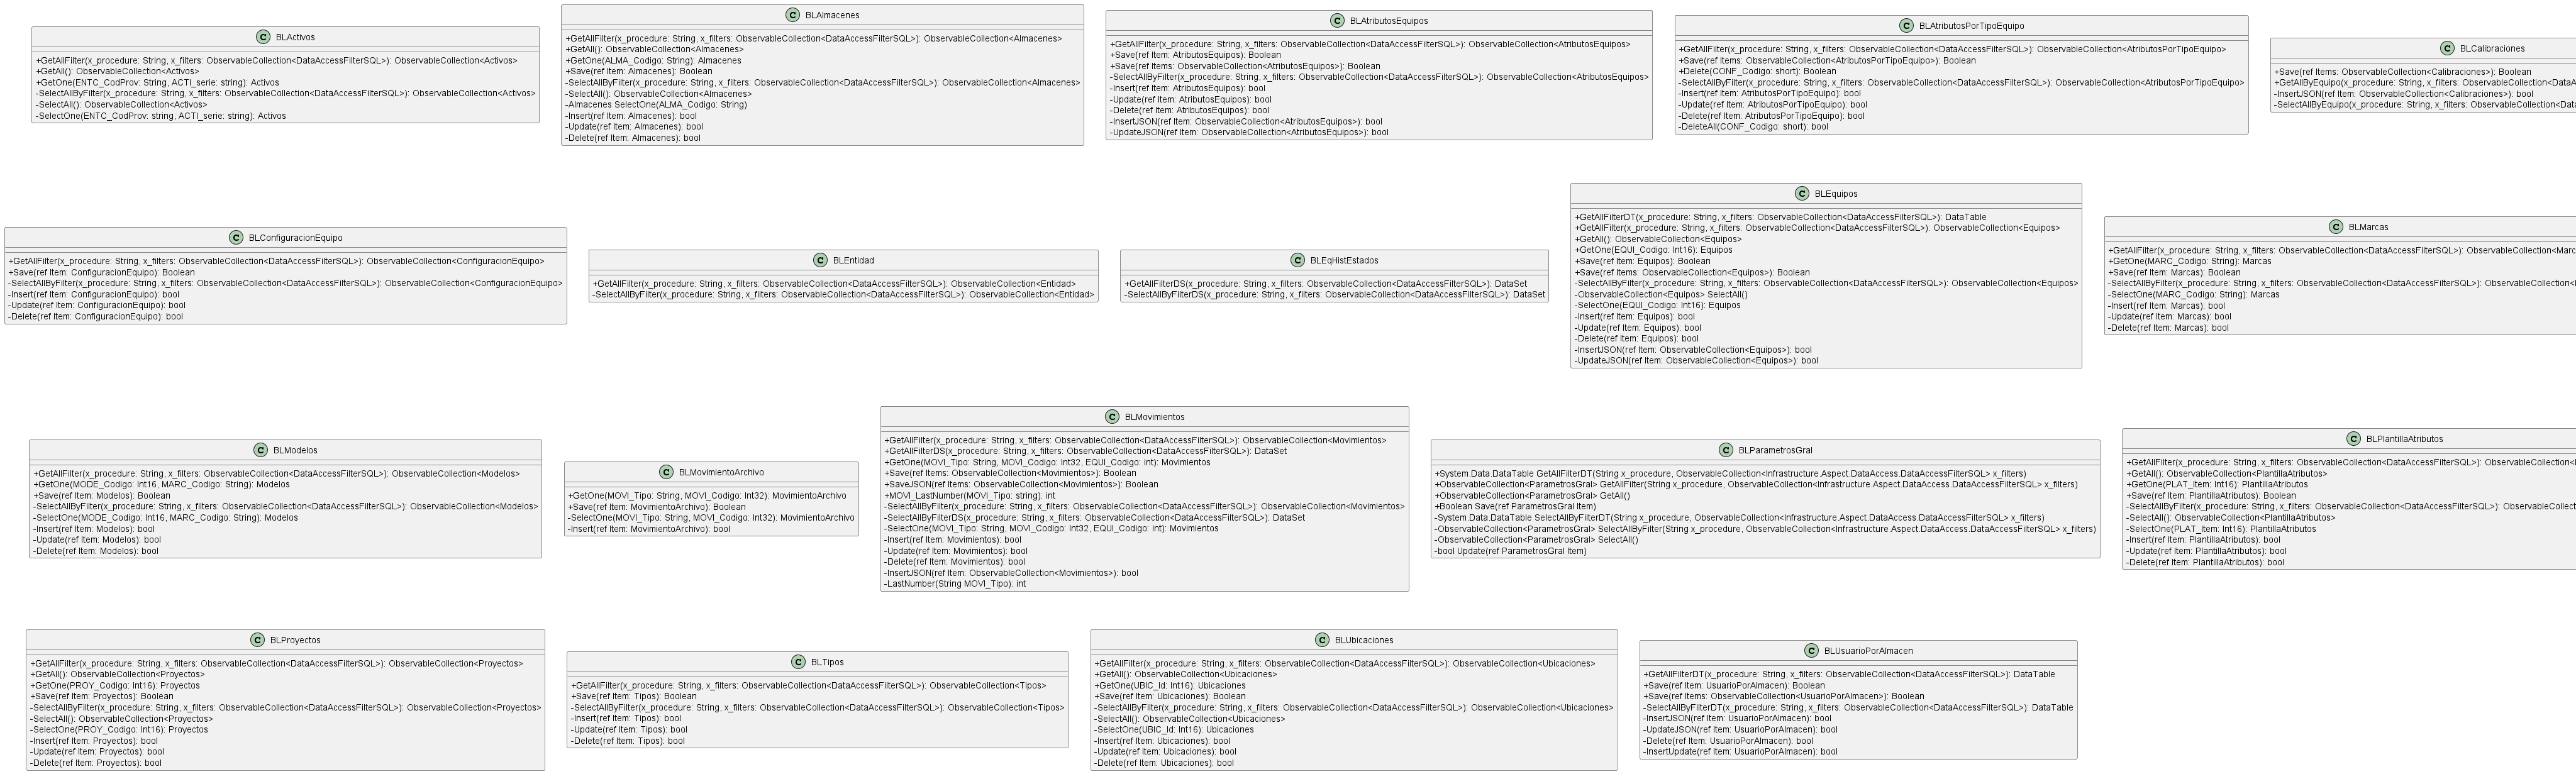
\includegraphics[width=21cm, height=16.5cm, angle=90]{./diagrams/Classes/BusinessLogic/BusinessLogic.pdf}
\end{figure}
\begin{figure}[H]
    \centering
    \caption{Clases: API}
    \includegraphics[width=21cm, height=16.5cm, angle=90]{./diagrams/Classes/Services/Service.pdf}
\end{figure}
\subsubsection{Diagrama de Entidad Relación}
\begin{figure}[H]
    \centering
    \caption{Entidad Relación: Base de Datos}
    \includegraphics[width=21cm, height=16.5cm, angle=90]{./diagrams/ER/ER.pdf}
\end{figure}
\subsubsection{Diagramas de Secuencia}
\begin{figure}[H]
    \centering
    \caption{Secuencia: Registrar Equipo Individual}
    \includegraphics[width=21cm, height=16.5cm, angle=90]{./diagrams/Sequence/RegistrarEquipo/RegistrarEquipo.pdf}
\end{figure}
\begin{figure}[H]
    \centering
    \caption{Secuencia: Registrar Equipo de Forma Masiva}
    \includegraphics[width=21cm, height=16.5cm, angle=90]{./diagrams/Sequence/RegistrarEquipoMasivo/RegistrarEquipoMasivo.pdf}
\end{figure}
\begin{figure}[H]
    \centering
    \caption{Secuencia: Registrar Movimiento de Entrega de Equipos y Registrar Transferencia de Equipos entre Almacenes}
    \includegraphics[width=21cm, height=16.5cm, angle=90]{./diagrams/Sequence/EntregaTransferencia/EntregaTransferencia.pdf}
\end{figure}
\begin{figure}[H]
    \centering
    \caption{Secuencia: Registrar Movimiento de Devolución de Equipos}
    \includegraphics[width=21cm, height=16.5cm, angle=90]{./diagrams/Sequence/RegistrarDevolucion/RegistrarDevolucion.pdf}
\end{figure}
\subsubsection{Interfaces}
El diseño de la interfaz de usuario es importante para garantizar que los usuarios puedan interactuar de manera eficiente y efectiva con el
módulo de gestión de inventario de equipos. Ahora se presentarán mockups que representan las principales pantallas del módulo. Estos diseños
ayudarán a visualizar la disposición de los elementos en la interfaz y asegurarán que la experiencia del usuario sea intuitiva y coherente.

\textbf{Pantalla de Inicio de Sesión (Figura~\ref{login}). }La pantalla de inicio de sesión es la primera interacción del usuario con el
módulo. En esta pantalla, el usuario debe ingresar sus credenciales de NextSoft-ERP para acceder al sistema. La interfaz es sencilla, con
campos para el usuario y la contraseña, y un botón de inicio de sesión.
\begin{figure}[H]
    \centering
    \caption{Mockup: Inicio de Sesión}\label{login}
    
\includegraphics[width=16.5cm, angle=0]{./images/login.png}
\end{figure}
\textbf{Pantalla de Registro Individual de Equipo (Figura~\ref{individual}). }Esta pantalla permite al administrador registrar un nuevo equipo
en el sistema de forma individual. Incluye campos para ingresar detalles como el número de serie, modelo, marca, categoría, y otros atributos
específicos del equipo. Una vez completado el formulario, el administrador puede guardar el registro y automáticamente se generará un
movimiento de ingreso al almacén correspondiente.
\begin{figure}[H]
    \centering
    \caption{Mockup: Registrar Equipo Individual}\label{individual}
    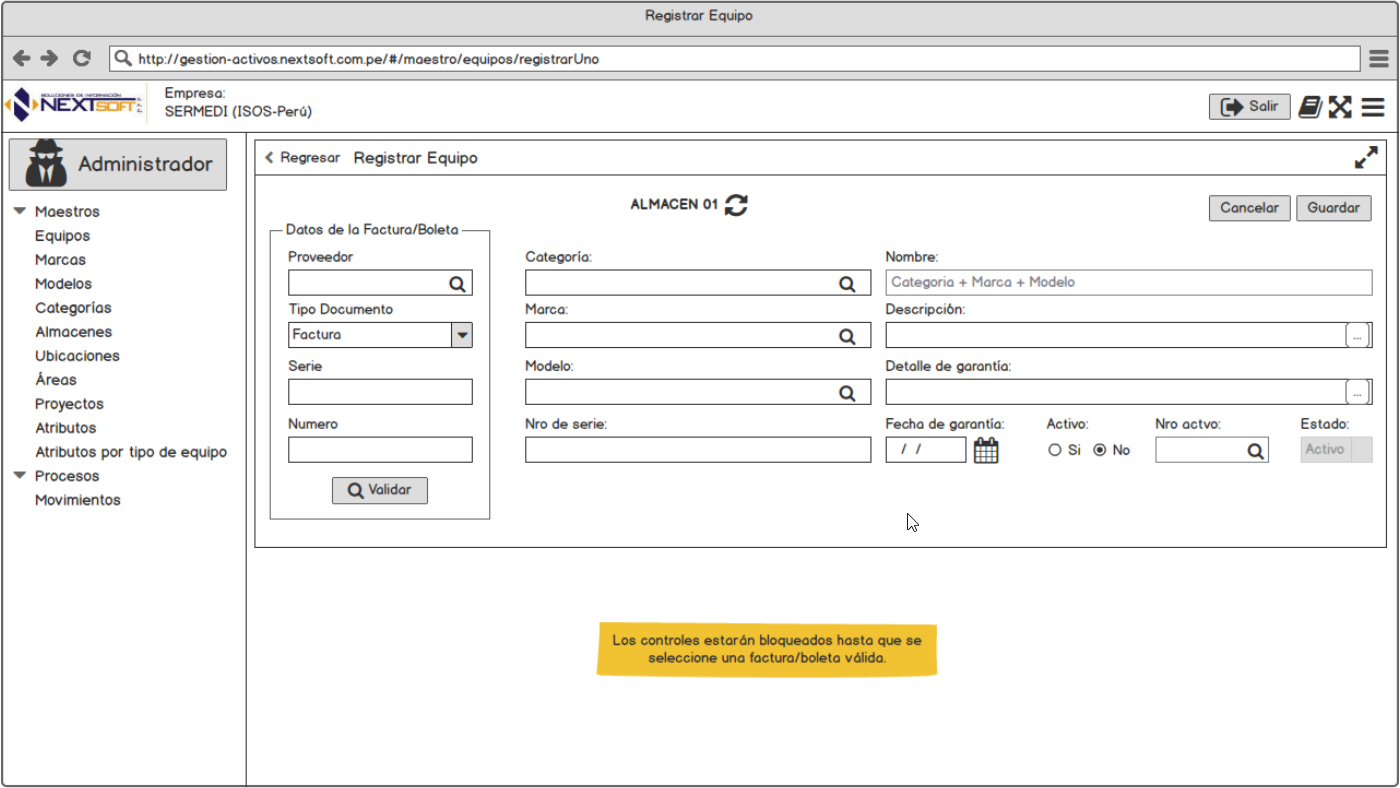
\includegraphics[width=16.5cm, angle=0]{./images/registroIndividual.png}
\end{figure}
\textbf{Pantalla de Registro Masivo de Equipos (Figura~\ref{masivo}). }La pantalla de registro masivo permite al administrador cargar un
archivo Excel que contenga los detalles de múltiples equipos. Esta interfaz incluye un área para seleccionar el archivo, una tabla con el
contenido del archivo, y botones para confirmar la carga y procesamiento de los datos. Los equipos registrados a través de esta funcionalidad
generarán movimientos de ingreso en el sistema.
\begin{figure}[H]
    \centering
    \caption{Mockup: Registrar Equipos Masivamente}\label{masivo}
    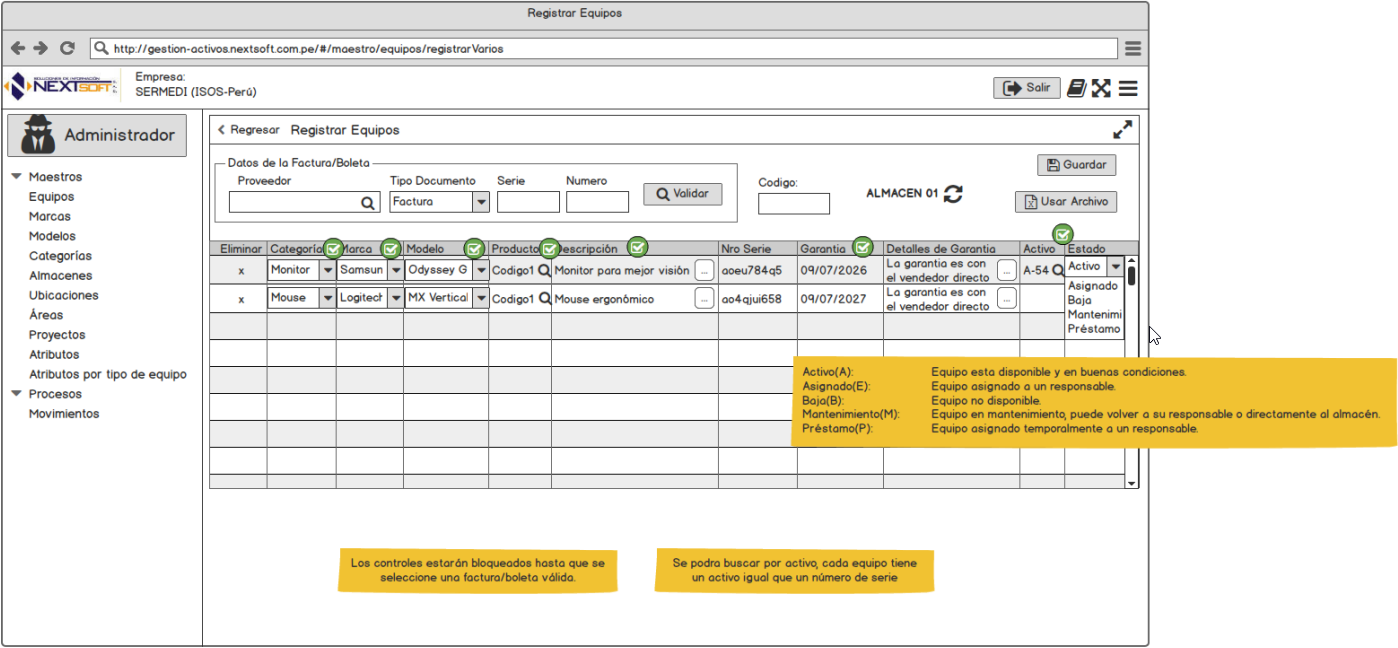
\includegraphics[width=16.5cm, angle=0]{./images/registroMasivo.png}
\end{figure}
\textbf{Pantalla de Registro de Entrega. }En la pantalla de registro de entrega, el administrador puede registrar la entrega de uno o varios
equipos a un responsable. La interfaz muestra una lista de equipos disponibles y permite seleccionar aquellos que serán entregados,
especificando el responsable y cualquier información adicional relevante. Una vez confirmada la entrega, los equipos seleccionados tendrán su
estado actualizado a ``Asignado''.
\begin{figure}[H]
    \centering
    \caption{Mockup: Registrar Movimiento (Primera Pestaña)}\label{movimiento1}
    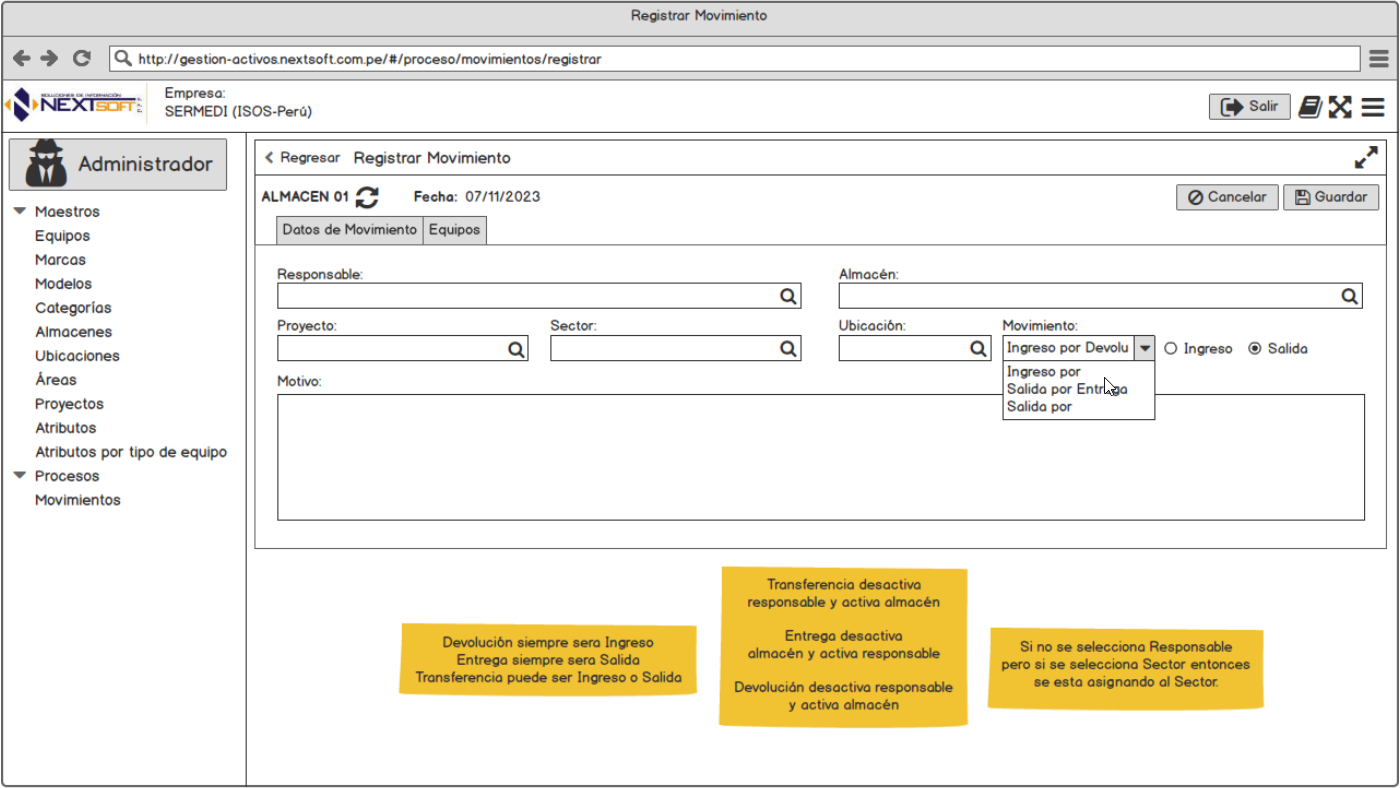
\includegraphics[width=10.4cm, angle=0]{./images/registrarMovimiento.png}
\end{figure}
\begin{figure}[H]
    \centering
    \caption{Mockup: Registrar Movimiento (Segunda Pestaña)}\label{movimiento2}
    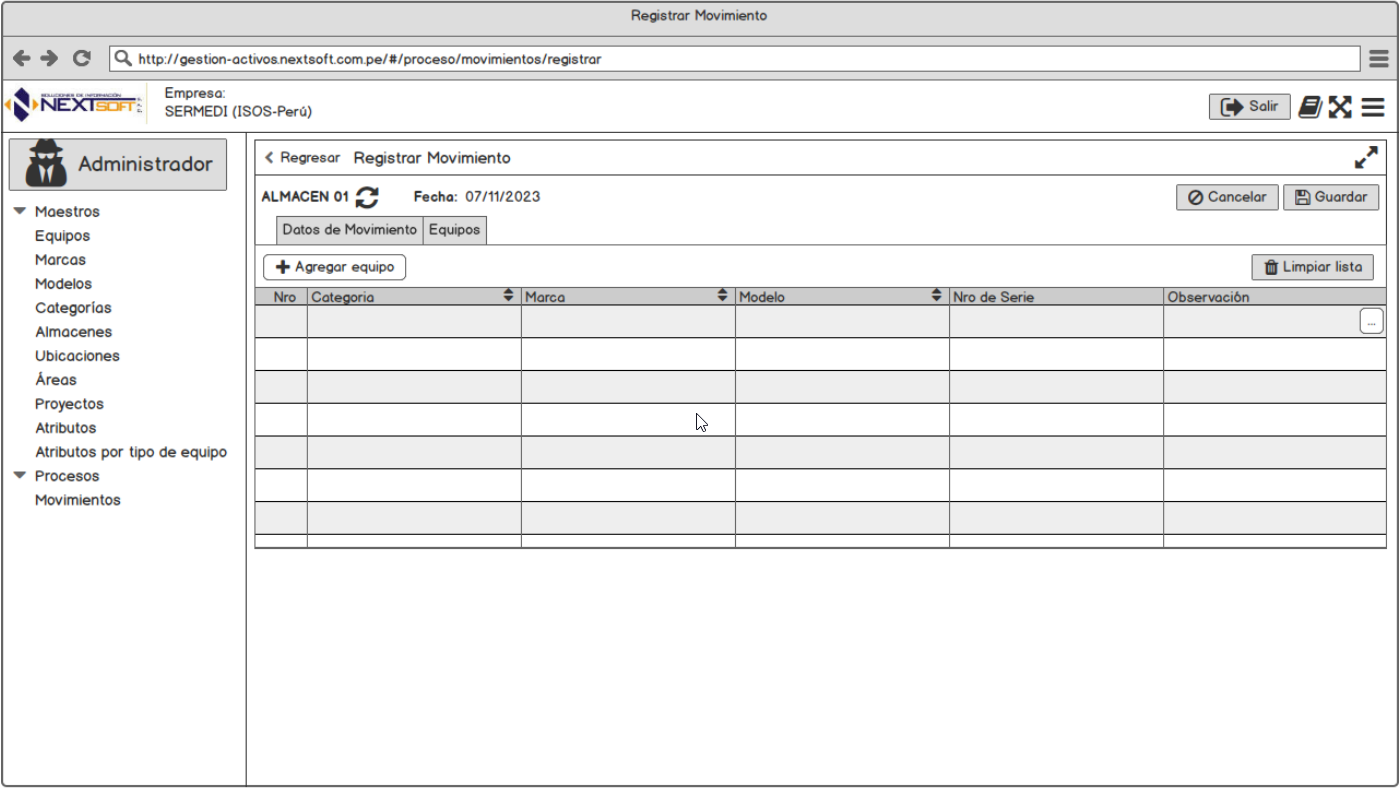
\includegraphics[width=16.5cm, angle=0]{./images/registrarMovimiento2.png}
\end{figure}
\textbf{Pantalla de Registro de Devolución. }Esta pantalla facilita el registro de la devolución de equipos al almacén. Similar a la pantalla
de entrega, se presentan los equipos que están actualmente asignados a responsables, y el administrador puede seleccionar los que se están
devolviendo. Al confirmar la operación, el estado de los equipos se actualiza a ``Disponible''.

\textbf{Pantalla de Registro de Transferencia. }La pantalla de registro de transferencia permite al administrador mover equipos de un almacén
a otro. La interfaz muestra los equipos disponibles en el almacén de origen, y el administrador selecciona los que se transferirán,
especificando el almacén de destino. Una vez completada la transferencia, se registran los movimientos correspondientes en el sistema y se
actualiza la ubicación de los equipos.
\subsubsection{Arquitectura}
La arquitectura del sistema resume cómo las diferentes capas interactúan entre sí para ofrecer una solución completa para la gestión de
inventario de equipos. La arquitectura está dividida en tres capas principales: la Capa de Presentación, la Capa de Lógica de Negocio y la
Capa de Acceso a Datos. Cada una de estas capas desempeña un papel crucial en el funcionamiento del sistema, asegurando la separación de
responsabilidades y facilitando el mantenimiento y la escalabilidad del módulo.

\textbf{Descripción de Capas. }

\textit{\textbf{Capa de Presentación (Angular 12). }}Esta capa es responsable de la interfaz de usuario (UI) y la experiencia del usuario (UX).
Desarrollada en Angular 12, la Capa de Presentación maneja la interacción del usuario con el sistema, permitiendo que los usuarios accedan a
las funcionalidades a través de una aplicación web responsiva. Angular 12 se comunica con la Capa de Lógica de Negocio mediante llamadas a la
API REST, enviando solicitudes y recibiendo datos para ser mostrados en la UI.

\textit{\textbf{Capa de Lógica de Negocio (.NET 8). }}La Capa de Lógica de Negocio está implementada en .NET 8 y es el núcleo del sistema,
gestionando todas las operaciones, reglas de negocio y validaciones. Esta capa está organizada en tres proyectos:
\begin{enumerate}
    \item\textbf{Service: } Este proyecto expone las funcionalidades del sistema a través de una API REST, permitiendo que la Capa de
          Presentación (Angular 12) interactúe con el sistema.
    \item\textbf{BusinessLogic: }Aquí se implementa la lógica de negocio, donde se gestionan todas las operaciones y procesos que el sistema
          debe realizar, como la gestión de equipos, movimientos, usuarios y configuración del sistema.
    \item\textbf{Entities: }Este proyecto contiene las entidades que representan los objetos de negocio, como Equipos, Almacenes, Movimientos,
          entre otros. Estas entidades son las que se manipulan en las operaciones de la lógica de negocio.
\end{enumerate}

\textit{\textbf{Capa de Acceso a Datos (SQL Server). }}La Capa de Acceso a Datos se encarga de interactuar con la base de datos SQL Server.
Desde la Capa de Lógica de Negocio, específicamente a través del proyecto BusinessLogic, se realizan las consultas y operaciones CRUD (Crear,
Leer, Actualizar, Eliminar) en la base de datos. SQL Server almacena toda la información relacionada con el inventario de equipos, incluyendo
sus atributos, movimientos, estados y configuraciones.

\textbf{Patrón de Diseño. }El sistema utiliza el patrón de diseño MVC (Model-View-Controller) para organizar el código y facilitar la
separación de responsabilidades. En este caso, Angular 12 actúa como la vista (View), presentando la información al usuario. La API REST
expuesta por~.NET 8 (Service) sirve como el controlador (Controller), gestionando las solicitudes del usuario y respondiendo con los datos
adecuados. Finalmente, las entidades y la lógica de negocio (Entities y BusinessLogic) representan el modelo (Model), donde se definen y
gestionan los datos y las reglas del negocio.
\subsubsection{Desarrollo}
En la implementación del módulo de gestión de inventario de equipos, se adoptó un enfoque ágil utilizando la metodología SCRUM, lo que permitió
una gestión eficiente y flexible del desarrollo. A pesar de que el proyecto fue realizado por un solo desarrollador, se estructuró de manera
que las tareas se organizaran y gestionaran de forma efectiva, similar a un entorno de desarrollo colaborativo.

\textbf{Metodología de Desarrollo. }Se utilizó SCRUM como marco de trabajo para gestionar el desarrollo del módulo. SCRUM, al ser una
metodología ágil, facilitó la adaptación continua a los cambios en los requerimientos y la retroalimentación constante. A través de la
implementación de sprints cortos y enfocados, se logró mantener un ritmo constante de avance, asegurando que cada incremento del producto
estuviera alineado con las necesidades del proyecto.

\textbf{Fases del Proyecto. }El desarrollo se dividió en 6 sprints, cada uno con una duración definida, lo que permitió una entrega incremental
del producto. Las fases principales incluyeron:
\begin{itemize}
    \item\textbf{Planificación: }Identificación de los requisitos del sistema y definición del backlog.
    \item\textbf{Diseño: }Creación de diagramas y diseño de la arquitectura del sistema.
    \item\textbf{Desarrollo: }Implementación de las funcionalidades del módulo, divididas en tareas manejables dentro de los sprints.
    \item\textbf{Pruebas: }Verificación de cada incremento del producto, asegurando que cumpliera con los criterios de aceptación.
    \item\textbf{Despliegue: }Integración del módulo con el sistema existente y preparación para el uso en producción.
\end{itemize}

\textbf{Gestión de Tareas. }Las tareas del proyecto fueron organizadas y gestionadas a través de Azure DevOps. Se definieron historias de
usuario para cada funcionalidad principal, y estas se dividieron en tareas individuales. A pesar de ser un solo desarrollador, el uso de
herramientas de gestión de proyectos como Azure DevOps permitió un seguimiento detallado del progreso, la priorización de tareas, y la
resolución de problemas a medida que surgían.

\textbf{Gestión de Código Fuente. }Se utilizó Subversion para la gestión del código fuente y la documentación del proyecto, garantizando que
cada cambio estuviera documentado y pudiera revertirse si fuera necesario.
\newpage
\section{Desarrollo e Implementación}
\subsection{Desarrollo del Módulo}
El desarrollo del módulo de gestión de inventario de equipos fue un proceso integral que involucró varias etapas técnicas, utilizando un
enfoque iterativo basado en la metodología SCRUM.~A continuación, se detallan los aspectos técnicos, las tecnologías empleadas, y el proceso
de desarrollo del módulo.
\subsubsection{Tecnologías Utilizadas.}
\textbf{Frontend. }El módulo fue desarrollado utilizando Angular 12, un framework que permite la creación de interfaces de usuario dinámicas,
responsivas y fáciles de mantener. Los componentes de la interfaz de usuario se diseñaron con una lógica de navegación clara y conexión a la
API REST del backend. Se hizo uso de servicios y módulos para organizar y reutilizar el código eficientemente.

\textbf{Backend. }Se utilizó~.NET 8 para implementar una API REST que interactúa con la base de datos y gestiona la lógica de negocio.~.NET 8
proporciona un entorno robusto para el desarrollo de aplicaciones empresariales, permitiendo una integración eficiente con el frontend.

\textbf{Base de Datos. }SQL Server se utilizó como el sistema de gestión de bases de datos para almacenar de manera segura y eficiente toda la
información relacionada con los equipos, movimientos, usuarios y configuraciones del módulo. SQL Server ofrece capacidades avanzadas de manejo
de datos, incluyendo transacciones, integridad referencial y consultas optimizadas.
\subsubsection{Estructura del Proyecto.}
\textbf{Capa de Presentación. }La capa de presentación se diseñó utilizando los principios de Angular 12, donde los componentes
(Código~\ref{componente}) se organizaron en módulos (Código~\ref{modulo}) para mantener la modularidad y escalabilidad de la aplicación. Los
componentes de la UI se encargan de manejar la interacción (Código~\ref{interaccion}) del usuario y de enviar las solicitudes al backend a
través de servicios especializados (Código~\ref{conexion}). Además, se implementó un sistema de enrutamiento (Código~\ref{enrutamiento}) para
gestionar la navegación entre las distintas vistas, y se utilizaron formularios reactivos (Código~\ref{formulario}) para capturar y validar
la información de manera eficiente.
\begin{lstlisting}[caption={Angular: Componente}\label{componente}, numbers=left, breaklines=true, basicstyle=\small]
@Component({
    selector: 'app-almacenes',
    templateUrl: './almacenes.component.html',
    styleUrls: ['./almacenes.component.css'],
})
export class AlmacenesComponent implements OnInit {
    constructor(
        private repositoryService: RepositoryService,
        private notificationService: NotificationService,
        private almacenesService: AlmacenesService
    ) { }
    ngOnInit() { }
}
\end{lstlisting}
\begin{lstlisting}[caption={Angular: Módulo}\label{modulo}, numbers=left, breaklines=true, basicstyle=\small]
@NgModule({
    imports: [
        AlmacenesRoutingModule,
    ],
    declarations: [AlmacenesComponent]
})
export class AlmacenesModule { }
\end{lstlisting}
\begin{lstlisting}[language=TeX, caption={Angular: Método en Componente}\label{interaccion}, numbers=left, breaklines=true, basicstyle=\small]
async GuardarAlmacen() {
    if (this.isSaving) {
        return;
    }
    this.isSaving = true;
    if (!this.almacenForm.valid) {
        this.notificationService.showInformationMessage('Verifica los campos obligatorios.');
        Object.keys(this.almacenForm.controls).forEach((controlName) => {
            const control = this.almacenForm.get(controlName);
            control?.markAsTouched();
        });
        this.isSaving = false;
        return;
    }
    const request: RequestRestGIV = {
        itemRequest: this.contextService.getRequest(),
        almacen: this.almacenForm.value || Almacen,
    };
    const apiresponse: ApiResponse = await this.repositoryService.AddAlmacen(request);
    if (apiresponse && apiresponse.Codigo == 0) {
        if (!request.almacen?.ALMA_CodPadre) {
            const request: RequestRestGIV = {
                itemRequest: this.contextService.getRequest(),
                almacen: this.searchForm.value as Almacen,
            };
            let ListadoAlmacenes = await this.repositoryService.GetAlmacenesPadre(request);
            this.almacenesService.SetAlmacenesPrincipal(ListadoAlmacenes);
            this.almacenes = this.almacenesService.GetAlmacenesPrincipal();
        }
        this.MView?.hide();
        this.notificationService.showSmallMessage('Se ha guardado el almacen.', true);
    }
    this.isSaving = false;
    await this.Buscar();
}
\end{lstlisting}
\begin{lstlisting}[language=TeX, caption={Angular: Conexión al Backend}\label{conexion}, numbers=left, breaklines=true, basicstyle=\small]
public CallService = (payload: any, method: string) => new Promise<any>((resolve) =>
    this.http.post<any>((this.url + method), payload, { headers: this.core.getDefaultOptions() })
    .subscribe(
        data => resolve(data),
        err => resolve(null)
    )
)
\end{lstlisting}
\begin{lstlisting}[language=TeX, caption={Angular: Enrutamiento}\label{enrutamiento}, numbers=left, breaklines=true, basicstyle=\small]
const routes: Routes = [
    {
        path: '',
        component: MainLayoutComponent,
        canActivate: [AuthGuard],
        children: [
            {
                path: 'maestros',
                loadChildren: () => import('src/app/features/maestros/maestros.module').then((m) => m.MaestrosModule),
            },
        ],
    },
    {
        path: 'auth',
        component: AuthLayoutComponent,
        loadChildren: () => import('src/app/features/auth/auth.module').then((m) => m.AuthModule),
    },
    { path: '**', redirectTo: 'auth' },
];
@NgModule({
    imports: [RouterModule.forRoot(routes)],
    exports: [RouterModule],
})
export class AppRoutingModule { }
\end{lstlisting}
\begin{lstlisting}[language=TeX, caption={Angular: Formulario Reactivo}\label{formulario}, numbers=left, breaklines=true, basicstyle=\small]
createAlmacenForm(Mview: boolean) {
    return new FormGroup({
        ALMA_Codigo: new FormControl('', []),
        ALMA_CodPadre: new FormControl('', []),
        ALMA_Nombre: new FormControl('', [Validators.required, Validators.maxLength(100)]),
        ALMA_Descripcion: new FormControl('', [Validators.required, Validators.maxLength(100)]),
        ALMA_Estado: new FormControl(true, [Validators.required]),
    });
}
\end{lstlisting}

\textbf{Capa de Lógica de Negocio. }

\textit{\textbf{Service. }}Los controladores API exponen los endpoints (Código~\ref{endpoint}) necesarios para que el frontend realice
operaciones CRUD (Crear, Leer, Actualizar, Eliminar) y otras interacciones con el sistema. Estos controladores gestionan las solicitudes HTTP
y se comunican con el proyecto BusinessLogic para ejecutar las acciones correspondientes.
\begin{lstlisting}[language=TeX, caption={.NET 8: Endpoint}\label{endpoint}, numbers=left, breaklines=true, basicstyle=\small]
[HttpPost("AddAlmacen")]
public ActionResult<Response> AddAlmacen([FromBody] RequestRestGIV request)
{
    Response _response = new Response();
    try
    {
        int _tiempodisponible = 0;
        if (ValidarSession(request.itemRequest.SESS_Token, request.itemRequest, ref _tiempodisponible))
        {
            BLAlmacenes BL_Almacen = new BLAlmacenes();
            Almacenes almacen = new Almacenes();
            request.almacen.CopyTo(ref almacen);
            almacen.Instance = Infrastructure.Aspect.BusinessEntity.InstanceEntity.Added;
            almacen.ALMA_Estado = true;
            almacen.AUDI_UsrCrea = request.itemRequest.USER_CodUsr;
            almacen.AUDI_HostCrea = request.itemRequest.AUDI_Host;
            if (BL_Almacen.Save(ref almacen))
            {
                _response.Mensaje = $"Se realizo correctamente el registro del almacen \"{request.almacen.ALMA_Nombre}\" con el ID {almacen.ALMA_Codigo}.";
                _response.Codigo = 0;
            }
            else
            {
                _response.Codigo = 1;
                _response.Mensaje = "Ha ocurrido un error al realizar el registro del almacen. </br>";
            }
            _response.TiempoSesion = _tiempodisponible;
        }
        else
        {
            _response.Codigo = 98;
            _response.Mensaje = string.Format("Mensaje: {0} - Tiempo Disponible: {1} minutos", "TOKEN No Valido", _tiempodisponible);
        }
    }
    catch (Exception ex)
    {
        String _code = Guid.NewGuid().ToString();
        _response.Codigo = 1;
        _response.Mensaje = string.Format("Error-{0}: {1}", _code, ex.Message);
        Util.WriteError(_code, ex, System.Reflection.MethodBase.GetCurrentMethod().Name);
    }
    return _response;
}
\end{lstlisting}

\textit{\textbf{BusinessLogic. }}Aquí se implementaron todas las reglas de negocio y validaciones necesarias para el correcto funcionamiento
del módulo. La lógica de negocio se organizó en métodos y clases (Código~\ref{bl}), permitiendo una separación clara de responsabilidades.
Esta capa interactúa directamente con la capa de acceso a datos para realizar operaciones sobre la base de datos.
\begin{lstlisting}[language=TeX, caption={.NET 8: Métodos de Business Logic}\label{bl}, numbers=left, breaklines=true, basicstyle=\small]
public partial class BLAlmacenes
{
    public Boolean Save(ref Almacenes Item)
    {
        try
        {
            Boolean m_isCorrect = true;
            switch (Item.Instance)
            {
                case InstanceEntity.Added:
                    m_isCorrect = Insert(ref Item); break;
                case InstanceEntity.Modified:
                    m_isCorrect = Update(ref Item); break;
                case InstanceEntity.Deleted:
                    m_isCorrect = Delete(ref Item); break;
            }
            return m_isCorrect;
        }
        catch (Exception)
        { throw; }
    }

    private bool Insert(ref Almacenes Item)
    {
        try
        {
            if (Item.Instance == InstanceEntity.Added)
            {
                SqlCommand DASqlCommand = DataAccessEnterpriseSQL.DAAsignarProcedure("GIV_ALMASI_UnReg");
                DataAccessEnterpriseSQL.DAAgregarParametro(DASqlCommand, "@ALMA_Codigo", Item.ALMA_Codigo, SqlDbType.VarChar, 6, ParameterDirection.InputOutput);
                DataAccessEnterpriseSQL.DAAgregarParametro(DASqlCommand, "@ALMA_CodPadre", string.IsNullOrEmpty(Item.ALMA_CodPadre) ? null : Item.ALMA_CodPadre, SqlDbType.VarChar, 6, ParameterDirection.Input);
                DataAccessEnterpriseSQL.DAAgregarParametro(DASqlCommand, "@ALMA_Nombre", Item.ALMA_Nombre, SqlDbType.VarChar, 100, ParameterDirection.Input);
                DataAccessEnterpriseSQL.DAAgregarParametro(DASqlCommand, "@ALMA_Descripcion", Item.ALMA_Descripcion, SqlDbType.VarChar, 100, ParameterDirection.Input);
                DataAccessEnterpriseSQL.DAAgregarParametro(DASqlCommand, "@ALMA_Estado", Item.ALMA_Estado, SqlDbType.Bit, 1, ParameterDirection.Input);
                DataAccessEnterpriseSQL.DAAgregarParametro(DASqlCommand, "@AUDI_UsrCrea", Item.AUDI_UsrCrea, SqlDbType.VarChar, 20, ParameterDirection.Input);
                DataAccessEnterpriseSQL.DAAgregarParametro(DASqlCommand, "@AUDI_HostCrea", Item.AUDI_HostCrea, SqlDbType.VarChar, 50, ParameterDirection.Input);
                if (DataAccessEnterpriseSQL.DAExecuteNonQuery(DASqlCommand, null) > 0)
                {
                    if (DASqlCommand.Parameters["@ALMA_Codigo"].Value != DBNull.Value && !String.IsNullOrEmpty(DASqlCommand.Parameters["@ALMA_Codigo"].Value.ToString()))
                    { Item.ALMA_Codigo = DASqlCommand.Parameters["@ALMA_Codigo"].Value.ToString(); }
                    return true;
                }
                else
                { return false; }
            }
            else
            { return true; }
        }
        catch (Exception)
        { throw; }
    }
}
\end{lstlisting}

\textit{\textbf{Entities. }}Las entidades (Código~\ref{entidad}) representan los datos clave dentro del sistema, como equipos, categorías,
movimientos, y usuarios. Estas entidades están definidas con sus respectivas relaciones, lo que permite una representación clara y
estructurada de la información en la base de datos.
\begin{lstlisting}[language=TeX, caption={.NET 8: Entidad}\label{entidad}, numbers=left, breaklines=true, basicstyle=\small]
public partial class Almacenes
{
    #region [ Variables ]
    private String m_alma_codigo;
    private String m_alma_codpadre;
    private String m_alma_nombre;
    private String m_alma_descripcion;
    private Nullable<Boolean> m_alma_estado;
    private String m_audi_usrcrea;
    private Nullable<DateTime> m_audi_feccrea;
    private String m_audi_hostcrea;
    private String m_audi_usrmod;
    private Nullable<DateTime> m_audi_fecmod;
    private String m_audi_hostmod;
    #endregion
    #region [ Constructores ]
    public Almacenes(){ }
    #endregion
    #region [ Propiedades ]
    [DataMember]
    public String ALMA_Codigo
    {
        get { return m_alma_codigo; }
        set
        {
            if (m_alma_codigo != value)
            {
                m_alma_codigo = value;
                OnPropertyChanged("ALMA_Codigo");
            }
        }
    }
    [DataMember]
    public String ALMA_CodPadre
    {
        get { return m_alma_codpadre; }
        set
        {
            if (m_alma_codpadre != value)
            {
                m_alma_codpadre = value;
                OnPropertyChanged("ALMA_CodPadre");
            }
        }
    }
    [DataMember]
    public String ALMA_Nombre
    {
        get { return m_alma_nombre; }
        set
        {
            if (m_alma_nombre != value)
            {
                m_alma_nombre = value;
                OnPropertyChanged("ALMA_Nombre");
            }
        }
    }
    [DataMember]
    public String ALMA_Descripcion
    {
        get { return m_alma_descripcion; }
        set
        {
            if (m_alma_descripcion != value)
            {
                m_alma_descripcion = value;
                OnPropertyChanged("ALMA_Descripcion");
            }
        }
    }
    [DataMember]
    public Nullable<Boolean> ALMA_Estado
    {
        get { return m_alma_estado; }
        set
        {
            if (m_alma_estado != value)
            {
                m_alma_estado = value;
                OnPropertyChanged("ALMA_Estado");
            }
        }
    }
    [IgnoreDataMember]
    public String AUDI_UsrCrea
    {
        get { return m_audi_usrcrea; }
        set
        {
            if (m_audi_usrcrea != value)
            {
                m_audi_usrcrea = value;
                OnPropertyChanged("AUDI_UsrCrea");
            }
        }
    }
    [IgnoreDataMember]
    [DisplayFormat(DataFormatString = "{0:yyyy-MM-dd}", ApplyFormatInEditMode = true)]
    public Nullable<DateTime> AUDI_FecCrea
    {
        get { return m_audi_feccrea; }
        set
        {
            if (m_audi_feccrea != value)
            {
                m_audi_feccrea = value;
                OnPropertyChanged("AUDI_FecCrea");
            }
        }
    }
    [IgnoreDataMember]
    public String AUDI_HostCrea
    {
        get { return m_audi_hostcrea; }
        set
        {
            if (m_audi_hostcrea != value)
            {
                m_audi_hostcrea = value;
                OnPropertyChanged("AUDI_HostCrea");
            }
        }
    }
    [IgnoreDataMember]
    public String AUDI_UsrMod
    {
        get { return m_audi_usrmod; }
        set
        {
            if (m_audi_usrmod != value)
            {
                m_audi_usrmod = value;
                OnPropertyChanged("AUDI_UsrMod");
            }
        }
    }
    [IgnoreDataMember]
    [DisplayFormat(DataFormatString = "{0:yyyy-MM-dd}", ApplyFormatInEditMode = true)]
    public Nullable<DateTime> AUDI_FecMod
    {
        get { return m_audi_fecmod; }
        set
        {
            if (m_audi_fecmod != value)
            {
                m_audi_fecmod = value;
                OnPropertyChanged("AUDI_FecMod");
            }
        }
    }
    [IgnoreDataMember]
    public String AUDI_HostMod
    {
        get { return m_audi_hostmod; }
        set
        {
            if (m_audi_hostmod != value)
            {
                m_audi_hostmod = value;
                OnPropertyChanged("AUDI_HostMod");
            }
        }
    }
    #endregion
    #region [ CopyTo ]
    public void CopyTo(ref Almacenes Item)
    {
        try
        {
            if (Item == null) { Item = new Almacenes(); }
            Item.ALMA_Codigo = this.ALMA_Codigo;
            Item.ALMA_CodPadre = this.ALMA_CodPadre;
            Item.ALMA_Nombre = this.ALMA_Nombre;
            Item.ALMA_Descripcion = this.ALMA_Descripcion;
            Item.ALMA_Estado = this.ALMA_Estado;
            Item.AUDI_HostCrea = this.AUDI_HostCrea;
            Item.AUDI_HostMod = this.AUDI_HostMod;
            Item.ALMA_NomPadre = this.ALMA_NomPadre;
        }
        catch (Exception ex)
        { throw ex; }
    }
    #endregion
}
\end{lstlisting}

\textbf{Capa de Acceso a Datos. }La capa de acceso a datos se implementó en el proyecto BusinessLogic, utilizando procedimientos almacenados
(Código~\ref{sp}) para ejecutar consultas a la base de datos. Esto permitió una interacción eficiente y segura con SQL Server, manteniendo la
lógica de acceso a datos separada de la lógica de negocio.
\begin{lstlisting}[language=TeX, caption={SQL Server: Procedimiento Almacenado}\label{sp}, numbers=left, breaklines=true, basicstyle=\small]
CREATE PROCEDURE dbo.GIV_ALMASI_UnReg 
    @ALMA_Codigo      VARCHAR(6) OUTPUT
  , @ALMA_CodPadre    VARCHAR(6)
  , @ALMA_Nombre      VARCHAR(100)
  , @ALMA_Descripcion VARCHAR(100)
  , @ALMA_Estado      BIT
  , @AUDI_UsrCrea     VARCHAR(20)
  , @AUDI_HostCrea    VARCHAR(50)  
AS  
BEGIN
    IF((SELECT ALMA_CodPadre 
          FROM GIV_Almacenes  
         WHERE ALMA_Codigo = @ALMA_CodPadre) IS NULL)  
        BEGIN  
            SET @ALMA_Codigo = ISNULL((SELECT MAX(CONVERT(INT,ALMA_Codigo))  
                                         FROM GIV_Almacenes), 0) + 1
            INSERT INTO GIV_Almacenes  
            ( ALMA_Codigo , ALMA_CodPadre , ALMA_Nombre , ALMA_Descripcion     
            , ALMA_Estado , AUDI_UsrCrea  , AUDI_FecCrea, AUDI_HostCrea    )  
            VALUES  
            ( @ALMA_Codigo, @ALMA_CodPadre, @ALMA_Nombre, @ALMA_Descripcion     
            , @ALMA_Estado, @AUDI_UsrCrea , GETDATE()   , @AUDI_HostCrea   )  
        END
    ELSE  
        BEGIN  
            RAISERROR('El almacen superior elegido no es valido, seleccione otro para continuar.', 18, 1)  
            RETURN  
        END  
END
\end{lstlisting}
\subsubsection{Proceso de Desarrollo.}
\textbf{Metodología de Desarrollo. }El proyecto fue gestionado utilizando la metodología ágil SCRUM, lo que permitió un desarrollo iterativo y
adaptable. A lo largo de los seis sprints, se realizó un seguimiento continuo del progreso y se ajustaron las tareas según las necesidades
emergentes. La gestión de tareas y sprints se llevó a cabo en Azure DevOps y la versión del código fue controlada mediante Subversion,
asegurando un historial claro de cambios y la capacidad de revertir a versiones anteriores si era necesario.

\textbf{Desarrollo Iterativo. }El módulo se desarrolló en seis sprints, cada uno con un objetivo claro y específico:
\begin{enumerate}
    \item\textbf{Análisis y diseño: }Se realizó el análisis de requerimientos y el diseño de mockups.
    \item\textbf{Desarrollo de mantenimiento de maestros: }Implementación de funcionalidades para la gestión de datos maestros.
    \item\textbf{Desarrollo de registro de equipos: }Creación de las funcionalidades para registrar equipos de manera individual y masiva.
    \item\textbf{Desarrollo de registro de movimientos: }Implementación de funcionalidades para registrar entregas, devoluciones y
          transferencias de equipos.
    \item\textbf{Desarrollo de reportes: }Creación de reportes detallados sobre equipos y movimientos.
    \item\textbf{Despliegue del módulo: }Despliegue final del módulo y preparación para su uso en el entorno de producción.
\end{enumerate}

\textbf{Pruebas Realizadas. }Las pruebas se realizaron en diferentes niveles para asegurar la calidad y funcionalidad del módulo:
\begin{itemize}
    \item\textbf{Pruebas del backend: }Utilizando Postman, se probaron exhaustivamente las APIs, verificando que respondieran correctamente y
          cumplieran con las especificaciones.
    \item\textbf{Pruebas del frontend: }Se realizaron pruebas en los formularios reactivos de Angular para asegurar que validaran correctamente
          la información obligatoria.
    \item\textbf{Pruebas de integración: }Se verificó que la comunicación entre el frontend y el backend funcionara sin problemas, incluyendo
          pruebas de guardado y recuperación de datos desde la base de datos.
    \item\textbf{Pruebas de guardado y recuperación de la base de datos: }Se llevaron a cabo pruebas para asegurar que los datos se guardaran
          y recuperaran correctamente en SQL Server, garantizando la integridad y consistencia de la información almacenada.
    \item\textbf{Pruebas de usuario: }Se llevaron a cabo pruebas de usuario para validar que el módulo cumpliera con los requerimientos y
          expectativas.
\end{itemize}
\subsection{Integración con Otros Sistemas}
\subsubsection{Integración con NextSoft-ERP}
\textbf{Autenticación. }El módulo utiliza el sistema NextAdmin para gestionar el inicio de sesión. Las credenciales de NextSoft-ERP,
proporcionadas a través del NextAdmin, permiten que solo usuarios autorizados accedan al módulo. Esta integración asegura que el acceso al
sistema esté restringido y que se mantenga la coherencia en la gestión de usuarios a través de los diferentes sistemas del ERP.

\textbf{Sincronización de Datos. }El módulo de gestión de inventario de equipos está diseñado para integrarse con varios sistemas del ERP.~Esto
incluye:
\begin{itemize}
    \item\textbf{Sistema de logística: }Se sincroniza con el sistema de logística para utilizar datos de marcas y productos. Esto garantiza
          que la información sobre los equipos sea precisa y esté alineada con las especificaciones definidas en el sistema de logística.
    \item\textbf{Sistema de activos: }Se conecta con el sistema de activos para obtener y relacionar datos de activos existentes. Esta
          integración permite una gestión más eficiente al asociar los datos de los activos con los equipos registrados en el módulo.
    \item\textbf{Sistema de tesorería: }El módulo se integra con el sistema de tesorería para acceder a comprobantes de compra, como boletas y
          facturas. Esto facilita la correcta asociación de los equipos con sus documentos de adquisición, asegurando que la información
          financiera y de inventario esté correctamente vinculada.
\end{itemize}
\subsubsection{Beneficios de la Integración}
\begin{itemize}
    \item\textbf{Optimización de procesos: }La integración con los sistemas de logística, activos, y tesorería facilita la automatización de
          procesos y reduce la duplicación de datos. Al sincronizar la información entre los sistemas, se minimiza la necesidad de ingresar
          datos manualmente y se asegura que la información esté actualizada en tiempo real. Esto contribuye a una gestión de inventario más
          eficiente y a una reducción de errores.
    \item\textbf{Mejora en la Toma de Decisiones: }La integración permite una visión más completa y precisa de la información relacionada con
          el inventario de equipos. Al tener acceso a datos consolidados de los sistemas de logística, activos y tesorería, los usuarios pueden
          tomar decisiones más informadas basadas en información actualizada y relevante. Esto facilita la planificación, el control y la toma
          de decisiones estratégicas relacionadas con el manejo de inventarios.
\end{itemize}
\newpage
\section{Resultados}
En esta sección se presentan los resultados obtenidos tras la implementación del módulo de gestión de inventario de equipos. Se describen los
aspectos más destacados del sistema, incluyendo su funcionamiento, interfaces desarrolladas, generación de reportes, y la integración con otros
sistemas dentro de la empresa.
\subsection{Implementación del Sistema}
A través de la API REST implementada en~.NET 8, el sistema permite una comunicación fluida y eficiente, asegurando un manejo robusto de la
lógica de negocio y acceso a los datos almacenados en SQL Server. La integración con NextSoft-ERP mediante el sistema NextAdmin garantiza que
la autenticación y autorización de los usuarios se gestionen de manera centralizada y segura.
\subsection{Interfaces Desarrolladas}
\subsubsection{Pantalla de Inicio de Sesión}
La pantalla de inicio de sesión [Figura~\ref{loginProd}] permite a los usuarios acceder al módulo utilizando sus credenciales de NextSoft-ERP,
gestionadas a través de NextAdmin. La autenticación centralizada asegura que solo los usuarios autorizados puedan acceder al sistema,
manteniendo la seguridad y el control de acceso.
\begin{figure}[H]
    \centering
    \caption{IU:~Inicio de Sesión}\label{loginProd}
    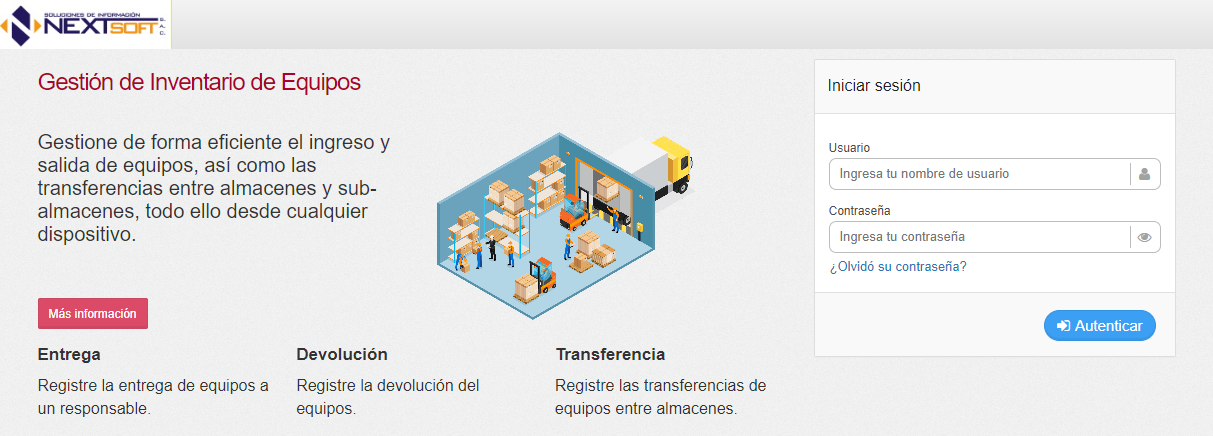
\includegraphics[width=16.5cm]{./images/loginProd.png}
\end{figure}
\subsubsection{Pantalla de Registro Individual de Equipo}
La interfaz para el registro individual de equipos [Figura~\ref{datosEquipo}] permite a los administradores ingresar detalladamente la
información de cada equipo, asi como sus atributos [Figura~\ref{atributosEquipo}] y sus calibraciones [Figura~\ref{calibracionesEquipo}],
asegurando que cada registro esté completo.
\begin{figure}[H]
    \centering
    \caption{IU:~Registro Individual de Equipo (Información)}\label{datosEquipo}
    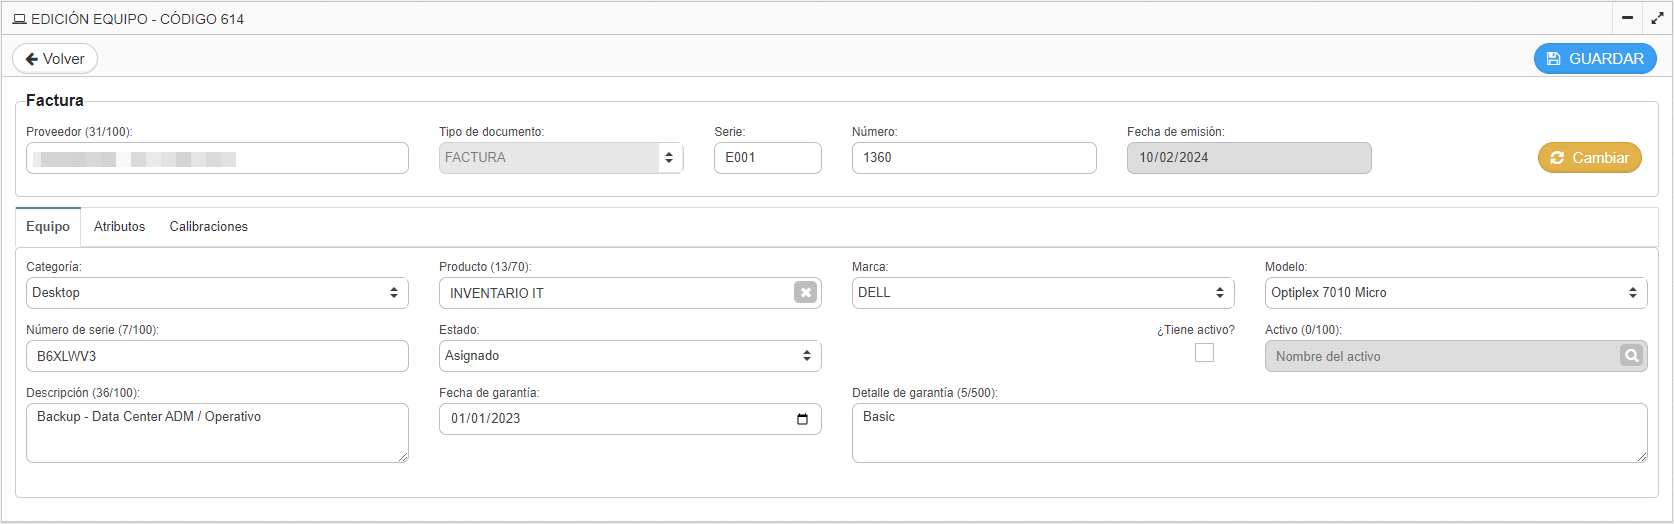
\includegraphics[width=16.5cm]{./images/datosEquipo.png}
\end{figure}
\begin{figure}[H]
    \centering
    \caption{IU:~Registro Individual de Equipo (Atributos)}\label{atributosEquipo}
    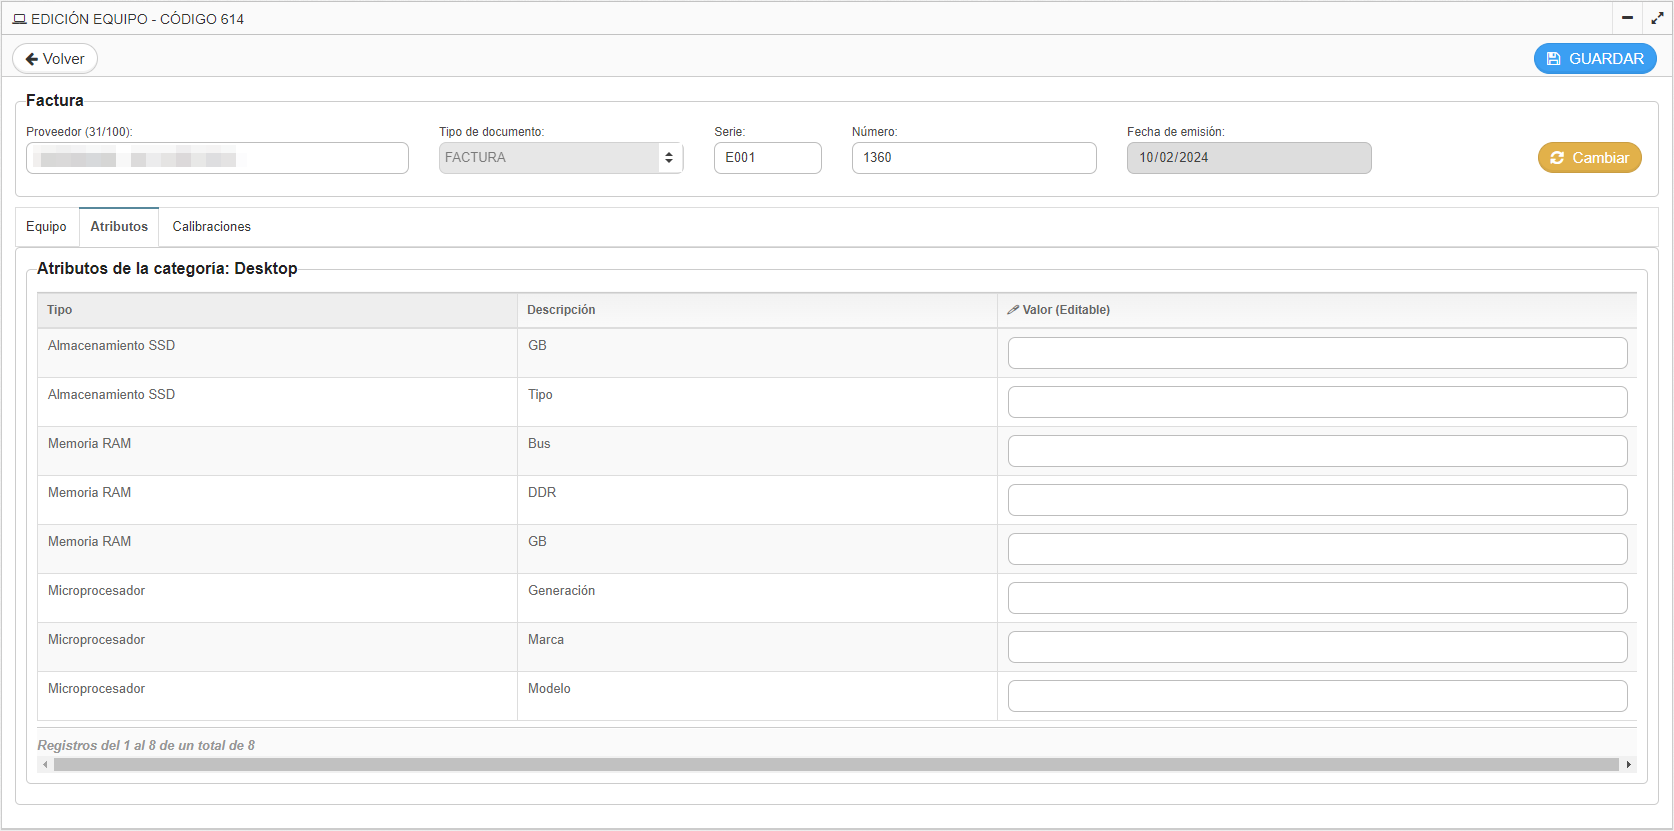
\includegraphics[width=16.5cm]{./images/equipoAtributos.png}
\end{figure}
\begin{figure}[H]
    \centering
    \caption{IU:~Registro Individual de Equipo (Calibraciones)}\label{calibracionesEquipo}
    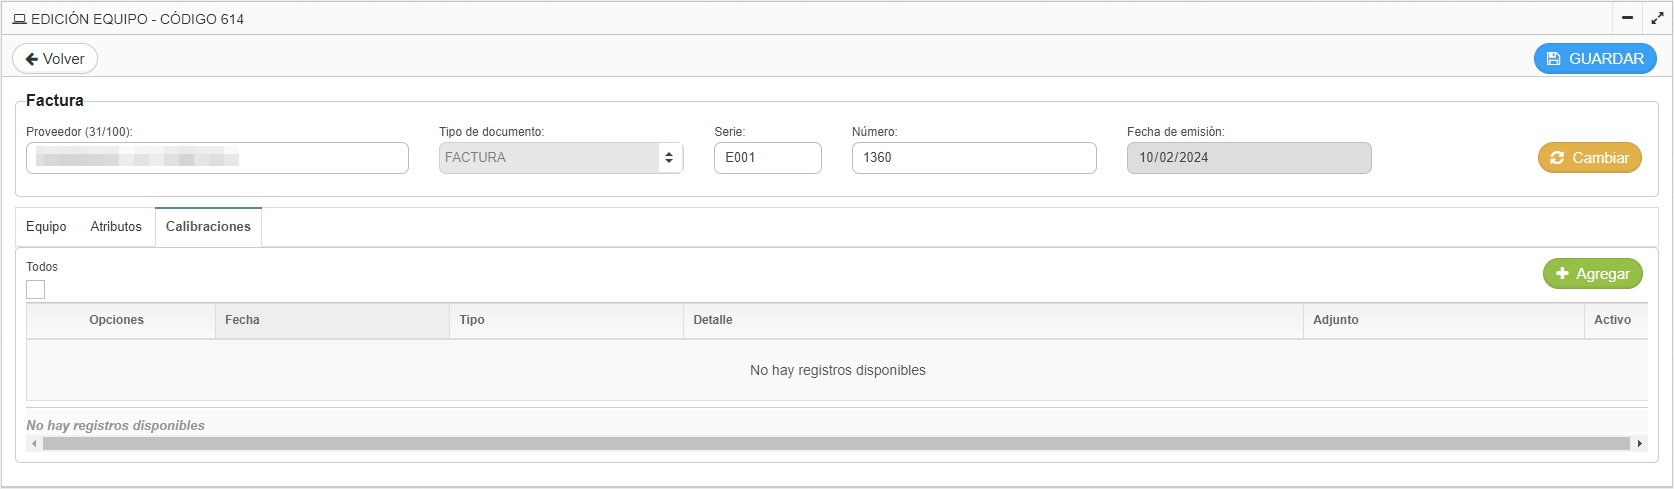
\includegraphics[width=16.5cm]{./images/calibracionesEquipo.png}
\end{figure}
\subsubsection{Pantalla de Registro Masivo de Equipos}
Para facilitar la carga de múltiples equipos, se desarrolló una interfaz para el registro masivo [Figura~\ref{equipoMasivo}], que permite al
administrador cargar un archivo Excel con los datos de los equipos. Esta funcionalidad agiliza el proceso de registro y minimiza el riesgo de
errores en la entrada de datos.
\begin{figure}[H]
    \centering
    \caption{IU:~Registro Masivo de Equipos}\label{equipoMasivo}
    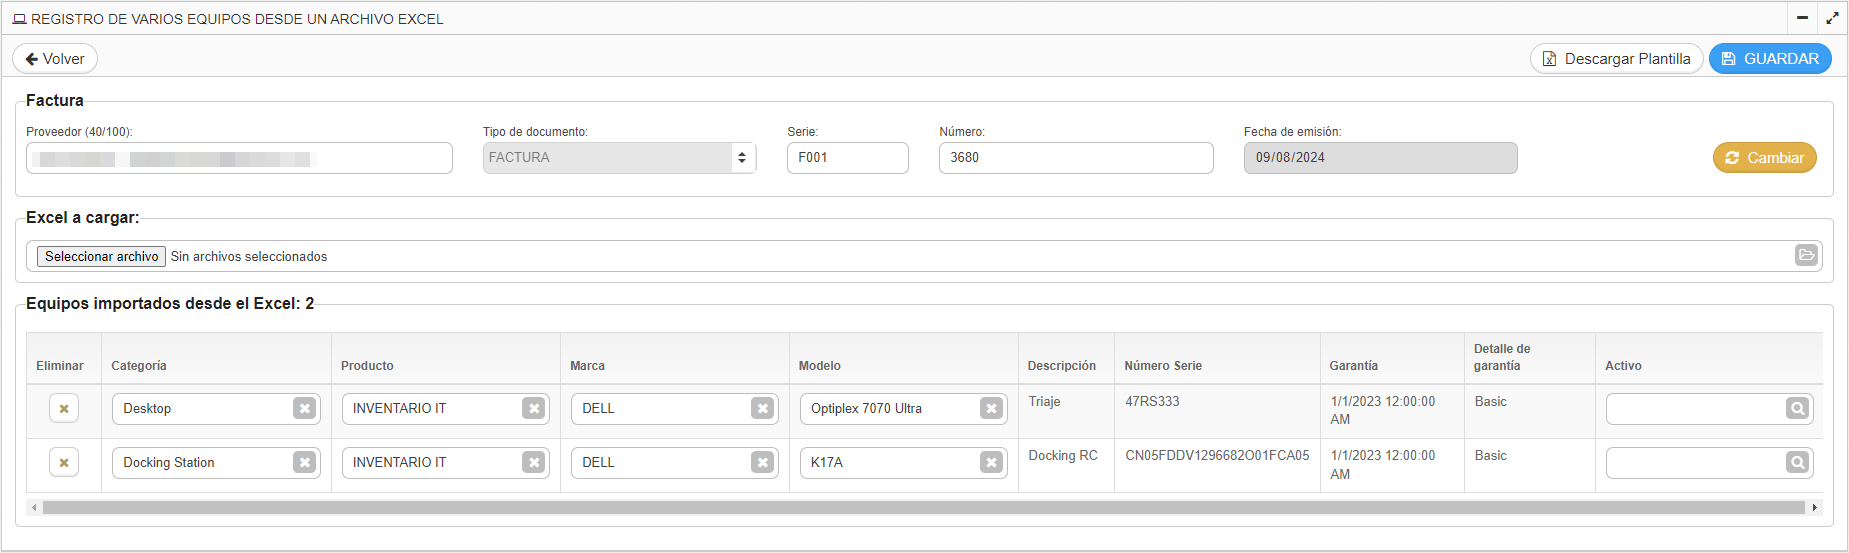
\includegraphics[width=16.5cm]{./images/equipoMasivo.png}
\end{figure}
\subsubsection{Pantalla de Registro de Entregas}
La interfaz de registro de entregas [Figura~\ref{entrega}] permite a los administradores documentar la entrega de equipos a los responsables
correspondientes. El estado de los equipos se actualiza automáticamente a ``Asignado'', garantizando que la información en el sistema esté
siempre actualizada.
\begin{figure}[H]
    \centering
    \caption{IU:~Registro de Entrega}\label{entrega}
    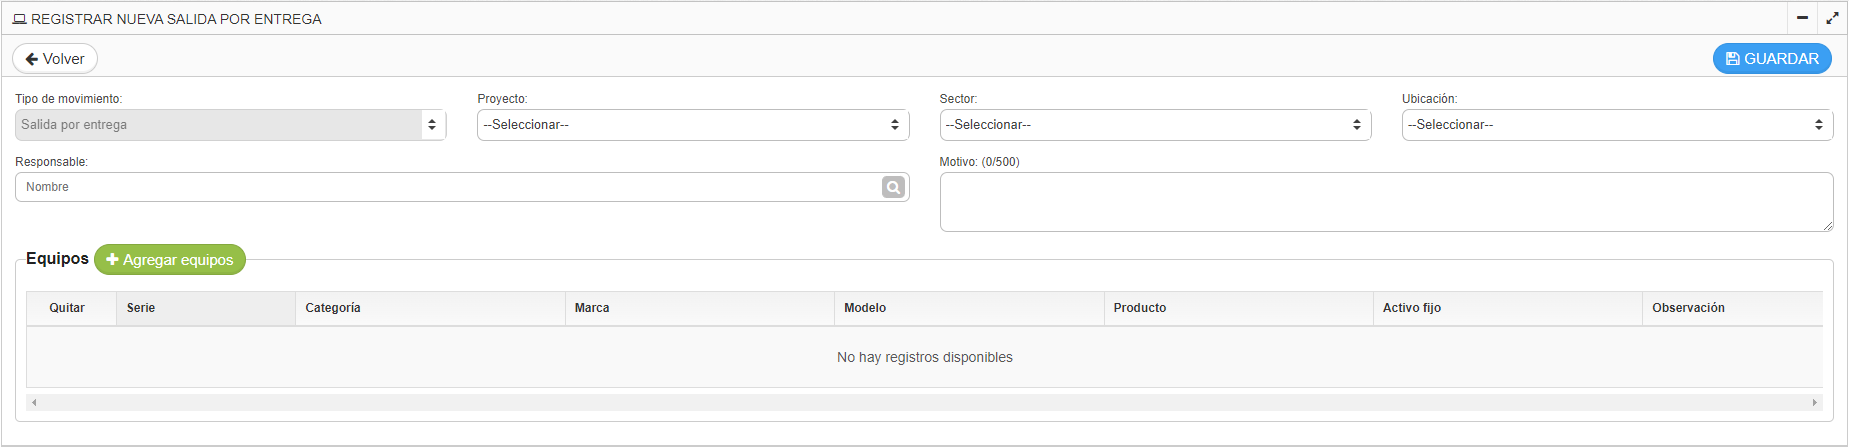
\includegraphics[width=16.5cm]{./images/entregaEquipo.png}
\end{figure}
\subsubsection{Pantalla de Registro de Devoluciones}
Similar a la entrega, la pantalla de registro de devoluciones [Figura~\ref{devolucion}] facilita la documentación de equipos que han sido
devueltos al almacén, actualizando su estado a ``Disponible''.
\begin{figure}[H]
    \centering
    \caption{IU:~Registro de Devolución}\label{devolucion}
    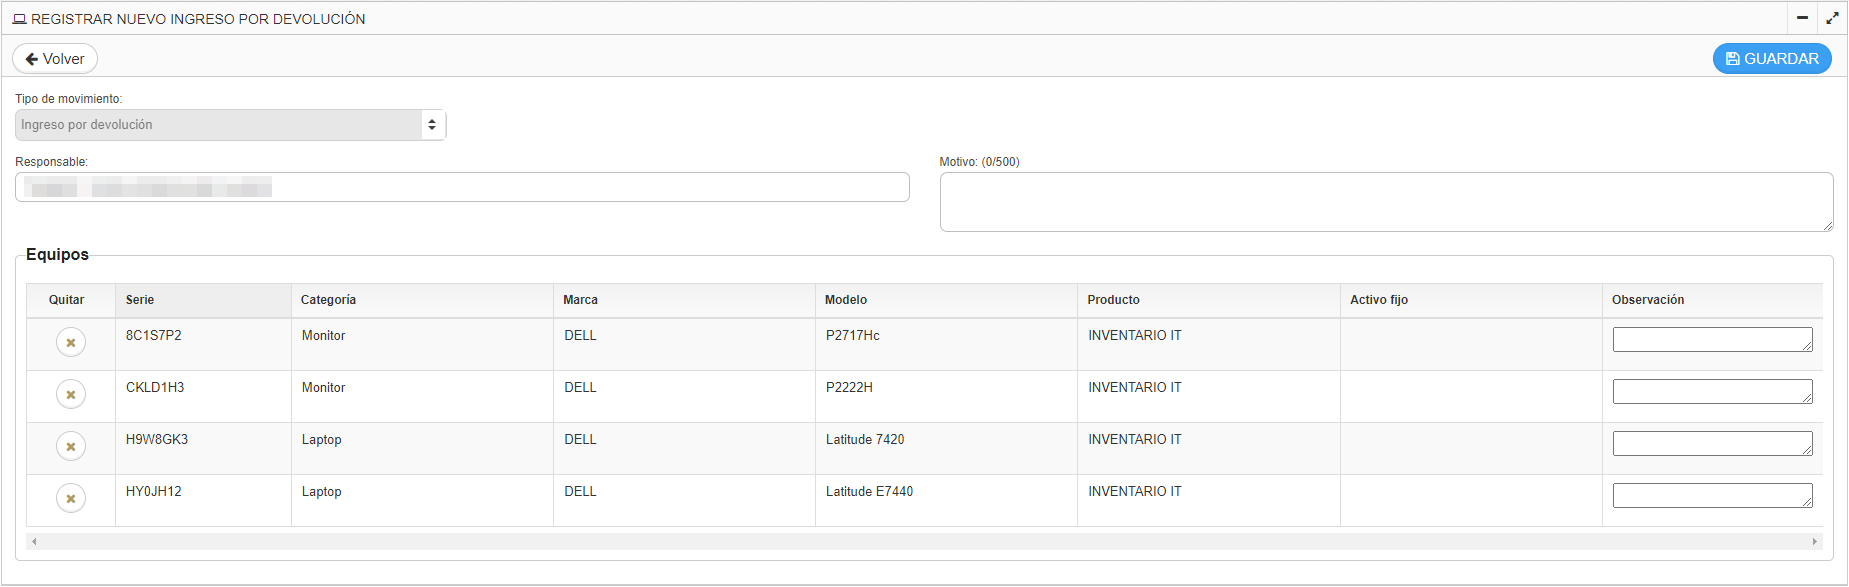
\includegraphics[width=16.5cm]{./images/devolucionEquipo.png}
\end{figure}
\subsubsection{Pantalla de Registro de Transferencias}
La pantalla para registrar transferencias [Figura~\ref{transferencia}] permite mover equipos de un almacén a otro, generando los movimientos
necesarios y asegurando que el inventario se mantenga preciso y sincronizado entre las diferentes ubicaciones.
\begin{figure}[H]
    \centering
    \caption{IU:~Registro de Transferencia}\label{transferencia}
    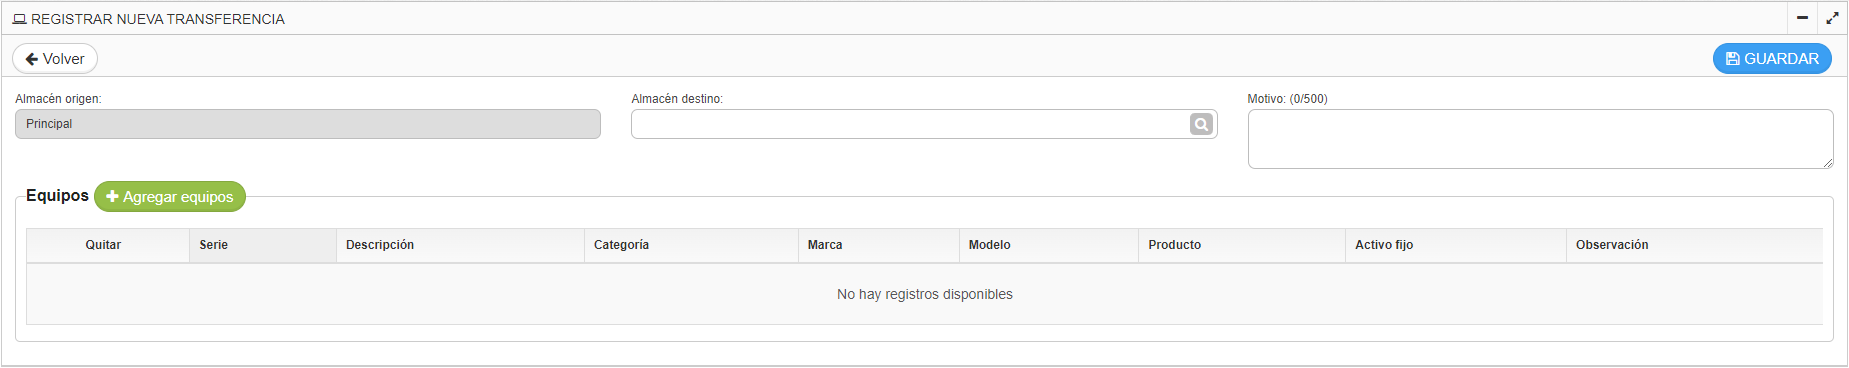
\includegraphics[width=16.5cm]{./images/transferencia.png}
\end{figure}
\subsection{Generación de Reportes}
El módulo cuenta con una funcionalidad de generación de reportes [Figura~\ref{reportes}] que permite a los usuarios crear informes detallados
y personalizables sobre el inventario de equipos. Estos reportes pueden filtrarse por múltiples criterios, como estado, categoría, almacén, y
otros parámetros relevantes, proporcionando una visión integral y precisa del inventario. Los reportes pueden ser exportados en formatos como
Excel, lo que permite un análisis detallado y la fácil presentación de la información. Además de estos reportes, cada movimiento realizado en
el sistema (como entregas, devoluciones y transferencias) genera un reporte específico, como cargos de entrega [Figura~\ref{cargoEntrega}],
cargos de devolución [Figura~\ref{cargoDevolucion}] y cargos de transferencia [Figura~\ref{cargoTransferencia}]. Estos documentos facilitan el
seguimiento y la documentación de cada operación.
\begin{figure}[H]
    \centering
    \caption{IU:~Reportes}\label{reportes}
    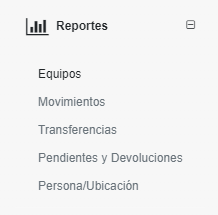
\includegraphics[scale=1]{./images/reportes.png}
\end{figure}
\begin{figure}[h]
    \caption{IU:~Cargos de Movimientos}\label{cargos}
    \centering
    \begin{subfigure}[b]{0.3\textwidth}
        \centering
        \caption{Cargo de Entrega}\label{cargoEntrega}
        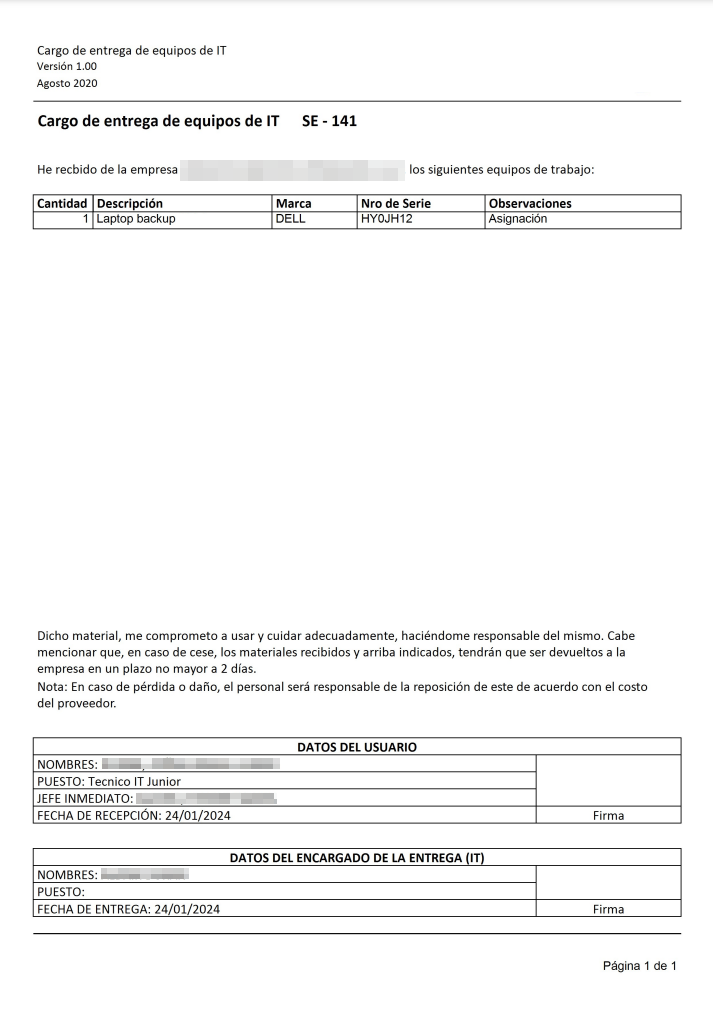
\includegraphics[width=\textwidth]{./images/reporteEntrega.png}
    \end{subfigure}
    \hfill
    \begin{subfigure}[b]{0.3\textwidth}
        \centering
        \caption{Cargo de Devolución}\label{cargoDevolucion}
        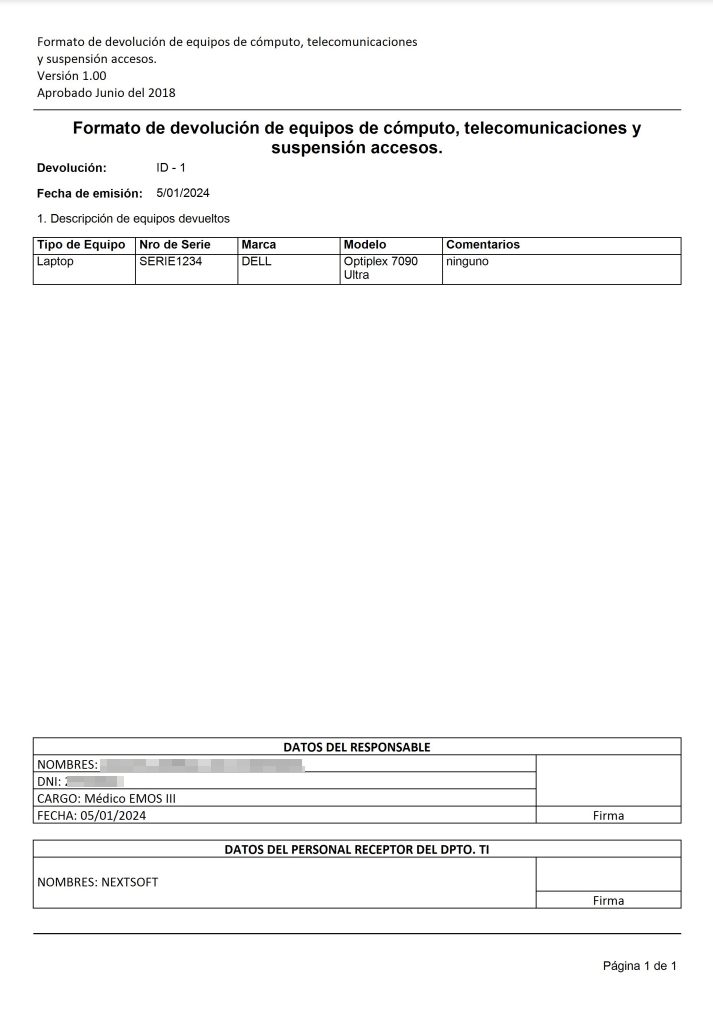
\includegraphics[width=\textwidth]{./images/reporteDevolucion.png}
    \end{subfigure}
    \hfill
    \begin{subfigure}[b]{0.3\textwidth}
        \centering
        \caption{Cargo de Transferencia}\label{cargoTransferencia}
        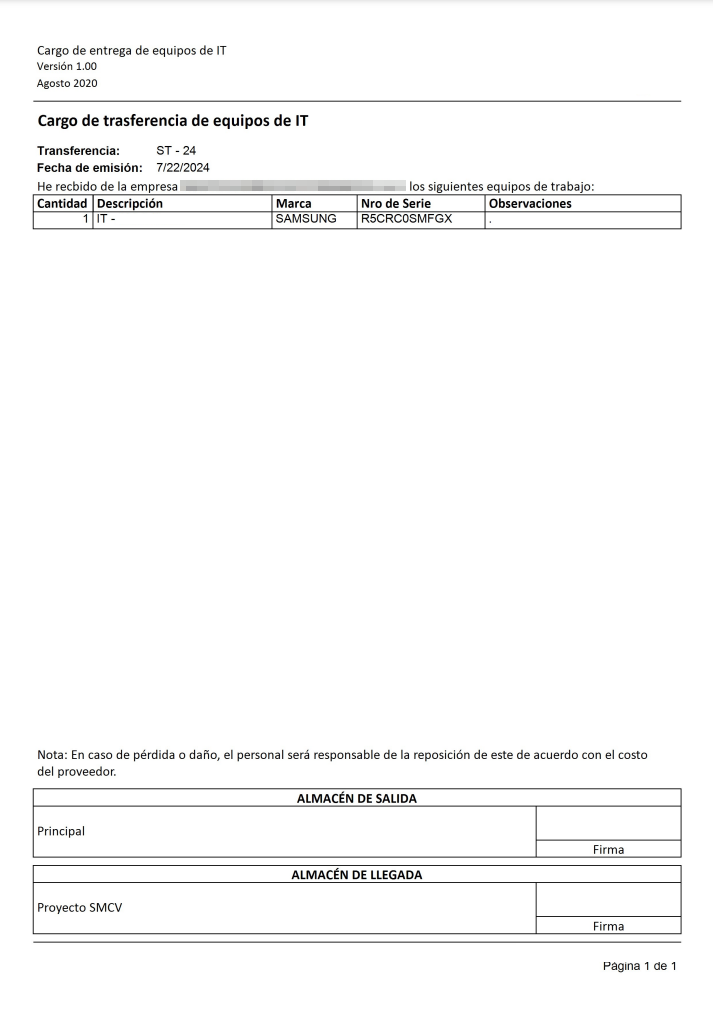
\includegraphics[width=\textwidth]{./images/reporteTransferencia.png}
    \end{subfigure}
\end{figure}

\newpage
\section{Conclusiones}
La implementación del módulo de gestión de inventario de equipos desarrollado para Soluciones de Información NextSoft S.A.C. ha demostrado ser
una solución robusta y eficiente, alineada con las necesidades operativas de la organización. El proyecto subraya la importancia de una
planificación cuidadosa y una ejecución rigurosa, utilizando una metodología ágil como SCRUM, que permitió un desarrollo adaptable a los
requerimientos cambiantes del entorno empresarial.
\begin{enumerate}
    \item % \subsection{Integración Exitosa con Sistemas Existentes}
          El módulo se integró eficazmente con los sistemas existentes de NextSoft-ERP, como el sistema de logística, el sistema de activos, y
          el sistema de tesorería. Estas integraciones no solo optimizaron los procesos de gestión de inventario, evitando la duplicación de
          datos y automatizando tareas, sino que también mejoraron la calidad y precisión de la información disponible para la toma de
          decisiones estratégicas.
    \item % \subsection{Arquitectura Técnica Solida}
          El diseño e implementación del módulo se llevaron a cabo utilizando tecnologías como Angular 12 para el frontend y~.NET 8 para el
          backend. La arquitectura multicapa, que incluye la capa de presentación, la capa de lógica de negocio, y la capa de acceso a datos,
          garantiza una clara separación de responsabilidades, facilitando tanto el mantenimiento como la escalabilidad del sistema. Además,
          el uso de procedimientos almacenados en SQL Server optimizó las operaciones de base de datos, asegurando una gestión eficiente y
          segura de los datos.
    \item % \subsection{Funcionalidades Clave y Experiencia de Usuario}
          El módulo ha proporcionado funcionalidades esenciales para la gestión de inventario de equipos, tales como el registro individual y
          masivo de equipos, la gestión de movimientos (entregas, devoluciones, y transferencias), y la generación de reportes detallados. La
          interfaz de usuario fue diseñada con un enfoque en la usabilidad, permitiendo a los usuarios interactuar con el sistema de manera
          intuitiva y productiva, garantizando una curva de aprendizaje mínima.
    \item % \subsection{Pruebas Exhaustivas y Aseguramiento de Calidad}
          Durante el desarrollo, se realizaron pruebas exhaustivas, utilizando herramientas como Postman para el backend y pruebas en formularios
          reactivos para el frontend. Estas pruebas aseguraron la calidad del sistema, verificando que la integración entre frontend y backend
          funcionara de manera correcta y confiable en producción. Asimismo, se garantizó la integridad de las operaciones de guardado y
          recuperación de datos desde la base de datos.
    \item % \subsection{Resultados y Beneficios}
          El módulo ha generado una mejora significativa en la gestión de inventario de equipos dentro de NextSoft. La capacidad para generar
          reportes detallados y específicos para cada tipo de movimiento ha proporcionado a la empresa una herramienta poderosa para el
          seguimiento y la auditoría de sus activos. Este proyecto representa un paso fundamental hacia la modernización y optimización de los
          procesos de gestión de inventario de la empresa, alineándose con las mejores prácticas de la industria y cumpliendo con altos
          estándares de calidad.
    \item % \subsection{Futuras Mejoras y Extensibilidad}
          Finalmente, la arquitectura del sistema y su integración con los sistemas existentes en NextSoft permiten futuras mejoras y extensiones,
          asegurando que el módulo pueda adaptarse a las necesidades cambiantes de la empresa y seguir aportando valor a largo plazo.
\end{enumerate}
\newpage
\section{Recomendaciones}
A partir de la experiencia adquirida durante el desarrollo e implementación del módulo de gestión de inventario de equipos para Soluciones de
Información NextSoft S.A.C., se presentan las siguientes recomendaciones para maximizar el aprovechamiento del sistema y facilitar futuras
mejoras:
\begin{enumerate}
    \item % \subsection{Capacitación Continua de los Usuarios}
          Aunque el sistema fue diseñado con un enfoque en la usabilidad y eficiencia, es recomendable llevar a cabo capacitaciones periódicas para los
          usuarios. Esto garantizará que todos los actores comprendan completamente las funcionalidades del sistema. La familiarización constante
          permitirá a los usuarios maximizar el uso de las capacidades del sistema.
    \item % \subsection{Monitoreo y Mantenimiento Regular del Sistema}
          Para asegurar el correcto funcionamiento del módulo a largo plazo, es esencial establecer un plan de monitoreo y mantenimiento regular. Esto
          incluye la supervisión del rendimiento del sistema, la actualización de las tecnologías utilizadas, como Angular y~.NET, y la optimización de
          la base de datos mediante la revisión periódica de los procedimientos almacenados. Mantener el sistema actualizado y en buen estado garantizará
          su eficiencia y seguridad continua.
    \item % \subsection{Extensión de Funcionalidades}
          Dado que el sistema ha sido diseñado con una arquitectura modular y escalable, se recomienda evaluar la posibilidad de extender sus
          funcionalidades en futuras fases. Ejemplos de mejoras podrían incluir la incorporación de un sistema de notificaciones automatizadas para
          alertar sobre eventos clave, como la llegada de equipos por transferencia, el vencimiento de la garantía de un equipo, o la implementación de
          la firma digital para cargos de movimientos realizados. Estas extensiones podrían incrementar aún más la eficiencia y el control sobre los
          activos.
    \item % \subsection{Revisión Periódica de la Seguridad del Sistema}
          La seguridad es un aspecto crítico, especialmente cuando se maneja información sensible. Se recomienda realizar auditorías de seguridad
          periódicas para identificar y mitigar posibles vulnerabilidades. Esto incluye la revisión de las políticas de autenticación, la protección de
          los datos en tránsito y en reposo, y la implementación de mecanismos de control de acceso más detallados, si fuera necesario. Un enfoque
          proactivo en la seguridad protegerá los activos de la empresa y la integridad de la información.
    \item % \subsection{Evaluación de la Satisfacción del Usuario}
          Para asegurar que el sistema continúa cumpliendo con las expectativas y necesidades de los usuarios, es recomendable realizar encuestas de
          satisfacción periódicas. Esto permitirá identificar áreas de mejora y ajustar el sistema en función de las experiencias y sugerencias de los
          usuarios finales, asegurando que el sistema evolucione con las necesidades del negocio.
    \item % \subsection{Documentación y Actualización Constante}
          Mantener una documentación actualizada y accesible es fundamental para la continuidad operativa y el mantenimiento del sistema. Esto incluye
          manuales de usuario, guías técnicas y documentación sobre la arquitectura del sistema. Una documentación bien mantenida facilita el proceso
          de mantenimiento y asegura la continuidad del conocimiento, incluso si el equipo de desarrollo cambia.
    \item % \subsection{Exploración de Nuevas Tecnologías}
          Finalmente, es recomendable estar atentos a la evolución de las tecnologías utilizadas en el proyecto. La rápida evolución de frameworks como
          Angular y plataformas como~.NET podría ofrecer nuevas herramientas y enfoques que mejoren el rendimiento, la seguridad y la usabilidad del
          sistema. Evaluar estas tecnologías y planificar actualizaciones garantizará que el sistema se mantenga a la vanguardia y continúe aportando
          valor.
\end{enumerate}
% \subsection{Mejora en la Integración con Otros Sistemas}
% Aunque la integración actual con los sistemas de logística, activos y tesorería de NextSoft-ERP ha sido exitosa, se recomienda explorar
% opciones para una integración más profunda. Por ejemplo, automatizar la actualización de inventarios en tiempo real o integrar el sistema con
% herramientas de análisis de datos podría proporcionar a la empresa una visión aún más completa y dinámica de su gestión de equipos.
% \newline
Siguiendo estas recomendaciones, NextSoft puede asegurarse de que el módulo de gestión de inventario de equipos siga siendo una herramienta
valiosa, eficaz y alineada con los objetivos estratégicos de la empresa, garantizando su relevancia y eficiencia a largo plazo.
\newpage
\bibliography{bibliography}
\nocite{*}
\end{document}
